% ============================================================================
% Chapter 4 — Methodology and Design
% Rubric-mandated two-section top level (4.1 and 4.2), followed by the
% theoretical analysis and the chapter signpost.
%
% Course outcome covered: CO5 (design alternatives, theoretical proofs).
% Figures specific to this chapter live in figures/ch4/; the detailed
% architecture figure is figures/system_architecture_figure.tex.
% ============================================================================

\chapter{Methodology and Design}
\label{ch:methodology}

% Chapter scope: Section 4.1 walks through the method at a high level and
% follows two real queries through it. Section 4.2 specifies every
% component, with the values used in the main run. Section 4.3 states the
% formal results and design heuristics, each labelled with its real status.

\section{Design Process or Methodology Overview}
\label{sec:design-process}

\subsection{The eight-stage pipeline narrative}
\label{sec:overview-pipeline}

CAEM answers each query with an eight-stage pipeline (\Cref{fig:system-architecture}). Stages 1 to 7 run once per query; Stage 8 runs once at the end of every cycle.
\begin{enumerate}
    \item \textbf{Pre-route:} a cheap confidence score $\upre$ is computed for the query before any answer is generated (\Cref{sec:pre-routing}).
    \item \textbf{Encode and look up:} the query is embedded and the nearest stored episode is found, giving a similarity $s$ and that episode's stored score $\ustored$ (\Cref{sec:gen-retrieval,sec:memory-store}).
    \item \textbf{Route:} the router picks one of three tiers from $s$, $\ustored$ and $\upre$ (\Cref{sec:router}). \textbf{Stage 3b:} when the router's choice would default to retrieval, the retrieval-utility classifier decides between retrieval and zero-shot generation (\Cref{sec:ruc}).
    \item \textbf{Answer:} Tier 1 returns the stored answer; Tier 2 generates without retrieval; Tier 3 retrieves Wikipedia passages and generates with them.
    \item \textbf{Verify:} every generated answer is scored by nine signals in four families (\Cref{sec:verifier}), which the calibrated composite turns into one probability of correctness, $\ustored$ (\Cref{sec:composite}).
    \item \textbf{Decide:} the four-outcome rule stores, defers, abstains or discards (\Cref{sec:conformal-gate,sec:decision}).
    \item \textbf{Output:} the user receives the answer with its calibrated probability and a reliability tag, or an insufficient-evidence message when the system abstains.
    \item \textbf{Cycle boundary:} the adapter is fine-tuned and checked for forgetting, the deferred buffer is revisited, the memory is consolidated, the composite is refitted and every stored episode is re-verified (\Cref{sec:cycle-boundary}).
\end{enumerate}

\subsection{The cycle loop walk-through}
\label{sec:overview-cycle}

A cycle has two phases. In the per-query phase, the pipeline answers a fresh stream chunk of $4{,}700$ training-panel questions (FEVER $2{,}000$, TriviaQA $2{,}000$, CommonsenseQA $700$). Each chunk shares no question with earlier chunks, with the calibration fold or with the evaluation fold. Answers that pass the storage gate enter the episodic memory and borderline answers enter the deferred buffer. The evaluation fold is then answered without writing to memory.

In the cycle-boundary phase, five steps run in a fixed order (\Cref{fig:cycle-boundary-order}). First, the low-rank adapter is fine-tuned on stored episodes whose $\ustored$ is at least $0.70$ and the retention guard checks three held-out probes; if any probe falls below $93$ percent of its starting accuracy, the previous adapter is restored and the remaining steps are skipped. Otherwise the deferred buffer is reconsidered, near-duplicate episodes are merged, the fixed calibration fold is re-scored with the new adapter so that the temperature and the composite can be refitted, and finally every stored episode is re-verified with the refitted composite. Re-verification can lower a stored score as well as raise it, and entries that fall below $0.50$ are removed. The memory itself is never rolled back: answers verified during a failed cycle stay in it.

% Cycle-boundary order as executed (outputs/full_run/experiment.log, e.g. cycle 2).
\begin{figure}[!htbp]
\centering
\resizebox{\textwidth}{!}{%
\begin{tikzpicture}[
  font=\small,
  st/.style={rectangle, rounded corners=4pt, line width=0.9pt, align=center, inner sep=4pt, text width=2.55cm, minimum height=2.1cm, draw=teal!65!black, fill=teal!7},
  gd/.style={diamond, aspect=1.6, line width=0.9pt, align=center, inner sep=1pt, draw=red!60!black, fill=red!6, font=\footnotesize},
  flow/.style={-{Stealth[length=2.2mm]}, line width=0.9pt, draw=black!65},
]
  \node[st] (a) at (0,0) {\textbf{1. Fine-tune}\\{\footnotesize LoRA adapter on stored episodes with $\ustored \ge 0.70$}};
  \node[gd] (g) at (3.35,0) {retention\\$\ge 0.93$?};
  \node[st] (b) at (6.7,0) {\textbf{2. Reconsider deferred}\\{\footnotesize promote, keep, or drop after two passes}};
  \node[st] (c) at (9.75,0) {\textbf{3. Consolidate}\\{\footnotesize merge near-duplicates (similarity $> 0.92$)}};
  \node[st] (d) at (12.8,0) {\textbf{4. Recalibrate}\\{\footnotesize re-score the calibration fold; refit temperature and composite}};
  \node[st] (e) at (15.85,0) {\textbf{5. Re-verify memory}\\{\footnotesize re-score every entry; remove if $\ustored < 0.50$}};
  \draw[flow] (a) -- (g); \draw[flow] (g) -- node[above, font=\scriptsize]{yes} (b);
  \draw[flow] (b) -- (c); \draw[flow] (c) -- (d); \draw[flow] (d) -- (e);
  \node[rectangle, rounded corners=3pt, draw=red!60!black, fill=red!4, align=center, font=\footnotesize, text width=6.2cm] (r) at (3.35,-2.35) {\textbf{no:} restore the previous adapter and skip steps 2 to 5; the memory is kept unchanged};
  \draw[flow] (g) -- (r);
\end{tikzpicture}}
\caption[Order of the cycle-boundary steps as executed.]{Order of the cycle-boundary steps as executed in the main run. After step 5 the next cycle begins by answering a fresh stream chunk with Stages 1 to 7. Cycle four took the rollback branch.}
\label{fig:cycle-boundary-order}
\end{figure}


\subsection{A worked example}
\label{sec:overview-worked-example}

Two real records from the main run show the pipeline end to end (\Cref{tab:worked-example}).

\textbf{A stored answer:} the TriviaQA question \emph{In what year (or century) was Michelangelo born?} arrived in the cycle-one stream chunk. Its pre-routing confidence ($0.522$) was above the safety floor, no stored episode was similar enough for Tier 1 or Tier 2, and the retrieval-utility classifier kept the default, so Tier 3 retrieved passages and the generator answered \emph{1475}, citing a passage that states the birth year. The sampled reasoning chains agreed ($s_{\text{avg}} = 0.992$) and entailed the answer ($p_{\text{entail}} = 0.939$), while the best passage gave only moderate support ($p_{\text{ground,max}} = 0.469$). The composite weighed these signals into $\ustored = 0.760$, above the storage cut-point of $0.60$, so the answer was stored and shown to the user as verified. It was correct.

\textbf{An abstention:} the TriviaQA question \emph{The song ``If I Ruled The World'' comes from which musical?} is in the evaluation fold. At cycle zero, with only the cold-start memory, it fell through to Tier 3, where the retrieved passages mention the song but not the musical, and the generator answered \emph{I do not know}. Every signal was low and the composite gave $\ustored = 0.127$. Because this is below the deferral cut-point of $0.45$ and the best passage supports the answer weakly ($p_{\text{ground,max}} = 0.112 < 0.20$), the decision was to abstain: the user receives the insufficient-evidence message with the probability shown, and nothing is stored. The gold answer is \emph{Pickwick}, so abstaining avoided a likely wrong answer.

\begin{table}[!htbp]
\centering
\small
\begin{tabular}{@{}lcc@{}}
\toprule
 & \textbf{Stored example} & \textbf{Abstained example} \\
Question & Michelangelo's birth year & ``If I Ruled The World'' \\
\midrule
Cycle, fold & 1, stream chunk & 0, evaluation fold \\
Tier & 3 & 3 \\
$\upre$ & $0.522$ & $0.659$ \\
$u_{\text{token}}$, $u_{\text{dropout}}$, $u_{\text{internal}}$ & $0.163$, $0.600$, $0.282$ & $0.022$, $0.800$, $0.111$ \\
$s_{\text{avg}}$ / $p_{\text{entail}}$ & $0.992$ / $0.939$ & $0.804$ / $0.115$ \\
$p_{\text{ground,max}}$ / $p_{\text{ground,mean}}$ & $0.469$ / $0.292$ & $0.112$ / $0.094$ \\
$q_{\text{a,rel}}$ & $0.515$ & $0.500$ \\
\midrule
$\ustored$ & $\mathbf{0.760}$ & $\mathbf{0.127}$ \\
Decision & store & abstain \\
Outcome & correct (\emph{1475}) & no answer (gold \emph{Pickwick}) \\
\bottomrule
\end{tabular}
\caption[Signal readings for the two worked examples.]{Signal readings for the two worked examples, read from the main run's per-sample records. The atomic-fact score equals the mean-passage score for both (\Cref{sec:verifier-grounding}).}
\label{tab:worked-example}
\end{table}

\section{Preliminary Design or Design (Model) Specification}
\label{sec:design-spec}

\begin{figure}[p]
\centering
\resizebox{\textwidth}{!}{%
\begin{tikzpicture}[
    xshift=-0.9cm,
    font=\normalsize,
  % ---- Node styles ----
  stage/.style  = {rectangle, draw=teal!65!black, line width=0.9pt, rounded corners=5pt,
                   minimum height=1.5cm, minimum width=6.5cm, align=center, fill=teal!8},
  router/.style = {rectangle, draw=teal!65!black, line width=0.9pt, rounded corners=5pt,
                   minimum height=1.8cm, minimum width=8.5cm, align=center, fill=yellow!18},
  mcyl/.style   = {cylinder, draw=teal!65!black, line width=0.9pt,
                   shape border rotate=90, aspect=0.25,
                   minimum height=3.0cm, minimum width=3.2cm, align=center, fill=teal!12},
  tA/.style     = {rectangle, draw=green!55!black, line width=1pt, rounded corners=5pt,
                   minimum height=1.7cm, minimum width=4.0cm, align=center, fill=green!12},
  tB/.style     = {rectangle, draw=red!55!orange, line width=1pt, rounded corners=5pt,
                   minimum height=1.7cm, minimum width=4.0cm, align=center, fill=red!12!orange!10},
  tC/.style     = {rectangle, draw=red!60!black, line width=1pt, rounded corners=5pt,
                   minimum height=1.7cm, minimum width=4.0cm, align=center, fill=red!10},
  verify/.style = {rectangle, draw=teal!65!black, line width=1pt, rounded corners=5pt,
                   minimum height=4.2cm, minimum width=9.5cm, align=center, fill=teal!5},
  decide/.style = {rectangle, draw=teal!65!black, line width=0.9pt, rounded corners=5pt,
                   minimum height=1.8cm, minimum width=9.5cm, align=center, fill=yellow!18},
  oServe/.style = {rectangle, draw=green!60!black, line width=1pt, rounded corners=4pt,
                   minimum height=1.4cm, minimum width=3.6cm, align=center,
                   fill=green!30, font=\small\scshape},
  oStore/.style = {rectangle, draw=green!60!black, line width=0.9pt, rounded corners=3pt,
                   minimum height=1.2cm, minimum width=2.7cm, align=center,
                   fill=green!28, font=\small\scshape},
  oDefer/.style = {rectangle, draw=green!45!black, line width=0.9pt, rounded corners=3pt,
                   minimum height=1.2cm, minimum width=2.7cm, align=center,
                   fill=green!12, font=\small\scshape},
  oAbst/.style  = {rectangle, draw=orange!75!black, line width=0.9pt, rounded corners=3pt,
                   minimum height=1.2cm, minimum width=2.7cm, align=center,
                   fill=orange!28, font=\small\scshape},
  oDisc/.style  = {rectangle, draw=red!60!black, line width=0.9pt, rounded corners=3pt,
                   minimum height=1.2cm, minimum width=2.7cm, align=center,
                   fill=red!28, font=\small\scshape},
  simp/.style   = {rectangle, draw=violet!60!black, line width=1pt, rounded corners=5pt,
                   minimum height=3.2cm, minimum width=17.0cm, align=center, fill=violet!7},
  % ---- Arrow styles ----
  farr/.style   = {-Latex, line width=0.9pt},
  garr/.style   = {-Latex, line width=1.1pt, green!50!black},
  oarr/.style   = {-Latex, line width=1.1pt, color=red!55!orange},
  rarr/.style   = {-Latex, line width=1.1pt, red!60!black},
  darr/.style   = {<->, dashed, line width=0.9pt, teal!55!black},
  varr/.style   = {-Latex, line width=1pt, dashed, violet!60!black},
    elab/.style   = {font=\small\itshape, inner sep=2pt, fill=none, draw=none}
]

% ==================================================================
% NODES   (main trunk centred at x = 6; y compressed to fit A4 page)
% ==================================================================

\node[stage]  (q)   at (6,   0.0)  {\textbf{Query $q$}};

\node[stage]  (s1)  at (6,  -2.5)  {%
    \textbf{S1\quad Pre-route confidence}\\[4pt]
    $u_{\text{pre}} = 0.60\,u_{\text{token}} + 0.40\,(1{+}C_{\text{conv}})^{-1}$\\
    {\scriptsize 32-token greedy decode $+$ one forward pass;\;$T$ refit per cycle}};

\node[stage]  (s2)  at (6,  -5.3)  {%
    \textbf{S2\quad Episodic memory retrieval}\\[4pt]
    SBERT 768-d cosine nearest-neighbour search};

% Episodic memory cylinder  (right of S2, connected by dashed bidirectional arrow)
\node[mcyl]   (mem) at (16.5,-5.3) {%
    \textbf{Episodic}\\[2pt]\textbf{Memory}\\[3pt]{\scriptsize exact search}};

\node[router] (s3)  at (6, -8.3)  {%
    \textbf{S3\quad Three-tier router}\\[4pt]
    $S(q)=0.70\cdot\mathrm{sim}(q,e^{*})+0.30\cdot u_{\text{stored}}(e^{*})$\\
    {\scriptsize safety override:\;if $u_{\text{pre}}<\phi_{\text{safe}}{=}0.38$ the score is bypassed and the RUC decides Tier~2 vs Tier~3}};

% ---- S3b: Retrieval-utility classifier (intercepts the safety-override and score-formula fall-throughs) ----
\node[router, minimum height=1.5cm, minimum width=5.0cm, fill=yellow!12]
      (ruc) at (16.5,-9.8) {%
    \textbf{S3b\quad RUC}\\[2pt]
    {\scriptsize 36-feature LR head;\;$p_{\text{RAG}}\gtrless\tau_{\text{RUC}}{=}0.375$}\\
    {\scriptsize routes safety-veto and else fall-through to Tier~2 or Tier~3}};

% ---- Tier row  (T1 far-left / T2 centre / T3 far-right)
%  S5 min-width = 9.5 cm centred at x=6  ->  left edge  ~ x = 1.25
%  T1 placed at x=0 is therefore outside S5, allowing a clean bypass path.
\node[tA] (t1) at (0.0, -12.2)  {%
    \textbf{Tier 1}\\[3pt]return $e^{*}$ answer\\{\scriptsize(from verified memory)}};
\node[tB] (t2) at (6.0, -12.2)  {%
    \textbf{Tier 2}\\[3pt]zero-shot generation\\{\scriptsize(fine-tuned generator, no retrieval)}};
\node[tC] (t3) at (12.0,-12.2)  {%
    \textbf{Tier 3}\\[3pt]retrieval-augmented\\{\scriptsize(top-5 Wikipedia passages)}};

% ---- S4: Tier execution grouping (compact left-side label; no wrapper) ----
\node[draw=none, inner sep=6pt, fit=(t1)(t2)(t3),
      label={[font=\small\bfseries, teal!65!black, anchor=east, xshift=-6pt]left:S4}]
     (s4box) {};

% Tier 1 direct-serve terminal  (left side, same y-band as S5)
\node[oServe] (serve) at (-3.5,-17.0) {%
    \textsc{Answer served}\\{\scriptsize from verified memory}};

% S5 centred at x=6, min-width=9.5 cm  ->  spans ~ x=1.25..10.75
\node[verify] (s5)  at (6, -17.0)  {%
    \textbf{S5\quad Nine-signal Verifier}\\[6pt]
    \textit{Internal:}\quad$u_{\text{token}},\;u_{\text{dropout}},\;u_{\text{internal}}$\\[3pt]
    \textit{Sample-set:}\quad$s_{\text{avg}},\;p_{\text{entail}}$\\[3pt]
    \textit{Grounding:}\quad$p_{\text{ground}}^{\max},\;p_{\text{ground}}^{\text{mean}},\;p_{\text{ground}}^{\text{atomic}}$\\[3pt]
    \textit{Relevance:}\quad$q_{\text{a,rel}}$\\[5pt]
    {\footnotesize\textbf{confabulation gate:}\;
     $u_{\text{internal}}{\geq}0.70\;\wedge\;p_{\text{ground}}^{\max}{\leq}0.20
     \;\Rightarrow\;$\textsc{Discard (early exit)}}};

\node[decide] (s6)  at (6, -21.0)  {%
    \textbf{S6\quad Four-outcome storage decision}\\[5pt]
    {\scriptsize
    $u_{\text{stored}}{\geq}0.60\Rightarrow\textsc{Store}$\quad
    $u_{\text{stored}}{\geq}0.45\Rightarrow\textsc{Deferred}$\quad
    $p_{\text{ground}}^{\max}{<}0.20\Rightarrow\textsc{Abstain}$\quad
    \textit{else:}\;\textsc{Discard}}};

% Terminal outcome boxes  (y = -24.5)
\node[oStore] (out1) at (2.0, -24.5)  {\textsc{Store}\\{\tiny write to memory}};
\node[oDefer] (out2) at (5.0, -24.5)  {\textsc{Deferred}\\{\tiny buffer; re-checked next cycle}};
\node[oAbst]  (out3) at (8.0, -24.5)  {\textsc{Abstain}\\{\tiny principled refusal}};
\node[oDisc]  (out4) at (11.0,-24.5)  {\textsc{Discard}\\{\tiny suppressed}};

% ---- S7: Memory write grouping (compact left-side label; no wrapper) ----
\node[draw=none, inner sep=6pt, fit=(out1)(out2)(out3)(out4),
      label={[font=\small\bfseries, teal!65!black, anchor=east, xshift=-6pt]left:S7}]
     (s7box) {};

% S8: between-cycle self-improvement  (wide band at bottom)
\node[simp] (s8) at (6, -27.5) {%
    \textbf{S8\quad Between-cycle self-improvement loop}
    \quad\textit{(runs once at each cycle boundary, not per query)}\\[6pt]
    (1)~Fine-tune the LoRA adapter on stored episodes with $\ustored{\geq}0.70$ (pool-reweighting layer; cross-entropy only)\\[3pt]
    (2)~Retention guard:\;worst probe ratio $\geq0.93$, else restore $\theta_{\text{prev}}$ and skip (3)--(5)\\[3pt]
    (3)~Reconsider deferred entries\quad(4)~Consolidate and recalibrate\quad
    (5)~Re-verify memory ($\ustored$ may rise or fall; remove below $\tau_{\text{retro}}{=}0.50$)};

% ==================================================================
% ARROWS
% ==================================================================

% ---- Main trunk ----
\draw[farr] (q.south)  -- (s1.north);
\draw[farr] (s1.south) -- node[elab,right]{$u_{\text{pre}}$} (s2.north);
\draw[farr] (s2.south) -- node[elab,right]{$u_{\text{pre}}$ + query embedding} (s3.north);

% ---- S2 <-> Episodic memory  (bidirectional dashed) ----
\draw[darr] (s2.east)
    -- node[elab,above,pos=0.55,align=center]{%
        retrieve $e^{*}$\;:\;$\mathrm{sim}(q,e^{*})$,\\$u_{\text{stored}}(e^{*})$}
    (mem.west);

% ---- S3 -> three tiers ----
\coordinate (br) at (6, -9.8);   % branch waypoint below S3
\draw[farr] (s3.south) -- (br);

% Tier 1 (green): branch LEFT, condition label above horizontal leg
\draw[garr]
    (br) --
    node[elab,above,pos=0.45]{\textbf{if}\;$S(q)\geq0.90$}
    (0.0,-9.8) -- (t1.north);

% Tier 2 (orange): straight down, condition label to the LEFT
\draw[oarr]
    (br) --
    node[elab,left,pos=0.5]{\textbf{elif}\;$\mathrm{sim}(q,e^{*})\geq0.75$}
    (t2.north);

% Score-formula else + safety-override both reach the RUC (S3b), not Tier 3 directly
\draw[farr]
    (br) --
    node[elab,above,pos=0.6]{\textbf{else}\;\textbf{or}\;$u_{\text{pre}}<\phi_{\text{safe}}$}
    (ruc.west);

% RUC -> Tier 3 (retrieval-augmented) when p_RAG >= tau_RUC
\draw[rarr]
    (ruc.south) --
    (ruc.south |- t3.east) --
    node[elab,above,pos=0.5]{$p_{\text{RAG}}\ge\tau_{\text{RUC}}$}
    (t3.east);

% RUC -> Tier 2 (zero-shot) when p_RAG < tau_RUC; direct diagonal to t2
\draw[oarr]
    (ruc.south west) --
    node[elab,above=2pt,sloped,pos=0.5]{$p_{\text{RAG}}<\tau_{\text{RUC}}$}
    (t2.north east);

% ---- Tier 1 bypass: route LEFT then DOWN, well outside S5 ----
% S5 left edge ≈ x=1.25; this path uses x=-3.5 to stay clear.
\coordinate (t1byp1) at (0.0, -14.0);    % just below T1
\coordinate (t1byp2) at (-3.5,-14.0);    % far left
\draw[garr]
    (t1.south) -- (t1byp1) --
    node[elab,below,pos=0.5]{\textit{bypass S5 and S6: episode already verified at storage time}}
    (t1byp2) -- (serve.north);

% ---- T2 -> S5 ----
\draw[oarr]
    (t2.south) --
    node[elab,right,pos=0.45]{answer + reasoning chain}
    (t2 |- s5.north);

% ---- T3 -> S5 routed on the right to avoid center-label overlap ----
\draw[rarr]
    (t3.south) --
    (12.0,-14.2) --
    (13.6,-14.2) --
    node[elab,right,pos=0.55]{answer + reasoning chain}
    (13.6,-16.9) --
    (s5.east);

% ---- S5 -> S6 ----
\draw[farr]
    (s5.south) --
    node[elab,right]{outputs:\;$u_{\text{stored}},\;p_{\text{contra}},\;p_{\text{ground}}^{\max}$}
    (s6.north);

% ---- S6 fan-out -> terminal boxes ----
\coordinate (br2) at (6,-22.8);
\draw[farr] (s6.south) -- (br2);
\draw[farr] (br2) -| (out1.north);
\draw[farr] (br2) -| (out2.north);
\draw[farr] (br2) -| (out3.north);
\draw[farr] (br2) -| (out4.north);

% ---- Store + Deferred accumulate into S8 at cycle end ----
% Drop only 0.3 cm so the horizontal segment stays ABOVE s8.north,
% then the vertical leg enters s8 cleanly from the top.
\draw[varr]
    (out1.south) -- ++(0,-0.3) -|
    node[elab,left,pos=0.05]{\textit{cycle end}}
    ($(s8.north)+(-2.5,0)$);
\draw[varr]
    (out2.south) -- ++(0,-0.3) -|
    ($(s8.north)+(-0.8,0)$);

% ---- S8 -> S1 : OUTER TEN-CYCLE LOOP ----
%
%  After S8 concludes, the updated weights θ_new (or θ_prev on rollback)
%  are loaded and Stage 1 of Cycle n+1 begins.  This arrow is the outer loop.
%
%  Route: S8.west  →  far left (x ≈ -5.5)  →  up to y of S1  →  S1.west
%
\draw[varr]
    (s8.west)
    -- ++(-5.5, 0) coordinate (ll)
    -- node[elab,left,pos=0.45,align=left]{%
        \textbf{Cycle $n{+}1$ begins}\\[3pt]
        S1 receives\\
        $\theta_{\text{new}}$ (fine-tuned)\\[1pt]
        or $\theta_{\text{prev}}$ (restored\\
        if abort guard fired)}
    (ll |- s1.west)
    -- (s1.west);

\end{tikzpicture}%
}
\caption[The eight-stage CAEM pipeline.]{The eight-stage CAEM pipeline. Stages S1 to S7 run once per query; S8 runs once per cycle, in the order of \Cref{fig:cycle-boundary-order}. The outer dashed arrow hands the updated or restored adapter to the next cycle.}
\label{fig:system-architecture}
\end{figure}


\subsection{Generator and retrieval substrate}
\label{sec:gen-retrieval}

Four components are fixed across every cycle.

\textbf{Generator:} Qwen2.5-3B-Instruct \cite{qwen25}, a three-billion-parameter instruction-tuned decoder, generates every Tier 2 and Tier 3 answer and supplies the internal-calibration signals. Only a low-rank adapter on top of it is trained (about $2$ percent of its parameters), which keeps each cycle's fine-tune within one $32$-gigabyte graphics processor. A small generator is also accurate enough on the training panel for the storage gate to have a usable signal.

\textbf{Retrieval corpus and encoder:} Tier 3 retrieves from a dense index of about $21$ million passages of roughly $100$ words from English Wikipedia, built in the dense-retrieval style of Karpukhin et al.~\cite{karpukhin-etal-2020-dense}. Queries, passages and memory entries are all embedded with the same sentence encoder, all-mpnet-base-v2 \cite{reimers-gurevych-2019-sentence} ($768$ dimensions), so a query can be compared directly with both. Tier 3 places the top five passages in the prompt. Both generating tiers ask the generator for a short reasoning followed by a line beginning \emph{Answer:}; the answer is read from that line, and the memory stores it together with the reasoning chain.

\textbf{Entailment judge:} MiniCheck-Flan-T5-Large \cite{tang2024minicheck} scores whether a premise supports a claim. It was trained on claim-support data generated by language models, which matches the kind of answers it is asked to judge. It returns a single support probability rather than a three-way label, so no contradiction signal is used. Inputs longer than its $512$-token encoder are truncated; a second, long-input judge built on the frozen generator was considered but dropped before the main run because its agreement with MiniCheck missed the required correlation floor (Pearson $0.584 < 0.70$, \Cref{ch:evaluation}).

\textbf{Reranker:} the cross-encoder bge-reranker-v2-m3 scores text pairs for relevance. The verifier uses it twice: to rerank the top $20$ retrieved passages down to the top three before entailment is scored, and to score how relevant the answer is to the question. Keeping the reranker separate from the entailment judge is what lets an off-topic answer that happens to be supported by an off-topic passage still be caught.

\subsection{Pre-routing confidence}
\label{sec:pre-routing}

The pre-routing confidence $\upre$ is a cheap estimate of how ready the generator is to answer, computed before any answer is produced. It feeds the safety override of the router. It combines two quantities (\Cref{alg:pre-routing}).

\textbf{Token confidence:} the generator runs a $32$-token greedy decode on the query and $u_{\text{token}}$ is the geometric mean of the probabilities of the tokens it chose. A model that hesitates between continuations scores low.

\textbf{Layer-convergence ratio:} one forward pass over the query records the hidden states of every decoder layer. The ratio $c_{\text{conv}}$ divides the variance of the hidden states in the first half of the layers by their variance in the second half, adapted from Nandakishor~\cite{nandakishor2025routing}. A large ratio means the representation is still unsettled in the early layers.

The two are combined with fixed weights, $z = 0.60\,u_{\text{token}} + 0.40/(1+c_{\text{conv}})$, and calibrated by temperature scaling \cite{pmlr-v70-guo17a} with a per-benchmark temperature $T_b$ fitted on the calibration fold. Temperature scaling was chosen because it has one parameter and preserves the order of scores.

\textbf{Realised behaviour:} on FEVER and TriviaQA the fitted temperature reached its upper bound ($T = e^{3} \approx 20.1$) at cycle zero and was refitted downward each cycle with exponential smoothing (to about $14$ at cycle one and $10$ at cycle two). A temperature this large pulls $\upre$ toward $0.5$, so on these benchmarks the score rarely approached the safety floor of $0.38$. \Cref{ch:evaluation} reports the consequence: the override fired on $63$ of the $9{,}000$ evaluation queries, $62$ of them on CommonsenseQA after its floor was refitted upward.

\begin{algorithm}[!htbp]
\caption[Pre-routing confidence (Stage~1).]{Pre-routing confidence (Stage~1).}
\label{alg:pre-routing}
\begin{algorithmic}[1]
\Require query $q$, generator $G$, decode length $L = 32$, per-benchmark temperature $T_{b}$
\State $(\log p_{1}, \dots, \log p_{n}) \gets$ log-probabilities of the tokens chosen by a greedy decode of up to $L$ tokens
\State $u_{\text{token}} \gets \exp\!\left(\tfrac{1}{n}\sum_{i=1}^{n} \log p_{i}\right)$ \Comment{geometric mean of token probabilities}
\State $\mathbf{H}^{(1)}, \dots, \mathbf{H}^{(D)} \gets$ hidden states of the $D$ decoder layers in one forward pass over $q$
\State $c_{\text{conv}} \gets \mathrm{Var}\big(\mathbf{H}^{(1:D/2)}\big) \,/\, \mathrm{Var}\big(\mathbf{H}^{(D/2+1:D)}\big)$ \Comment{early-half over late-half variance}
\State $z \gets 0.60\, u_{\text{token}} + 0.40\, /\,(1+c_{\text{conv}})$
\State \Return $\upre \gets \sigma\!\big(\mathrm{logit}(z)/T_{b}\big)$ \Comment{temperature scaling}
\end{algorithmic}
\end{algorithm}

\subsection{Episodic memory store}
\label{sec:memory-store}

The episodic memory is CAEM's long-term store of verified answers. It follows memory-augmented networks \cite{weston2015memory,graves2014neural,graves2016differentiable} and writeable episodic stores for language models \cite{larimar2024das,xu2025amem}, with one distinguishing feature: every entry carries the calibrated score $\ustored$ that admitted it.

\textbf{Record:} each entry holds the question, the answer, the reasoning chain, the question's embedding, the nine signal readings, $\ustored$, the source benchmark and the cycle in which it was stored. Keeping the question and answer together lets the cycle-boundary pass re-verify an entry without regenerating the answer.

\textbf{Cold start:} before cycle one, the pipeline answered questions from each training benchmark's seed pool until about $200$ per benchmark had been verified and stored ($603$ answers). Answers that were wrong against the gold labels were then removed, leaving $431$ entries (FEVER $155$, TriviaQA $136$, CommonsenseQA $140$). The cold-start memory is therefore correct by construction; every later entry is admitted by the verifier alone.

\textbf{Search:} lookup is by cosine similarity between question embeddings, because the encoder is trained to place paraphrases in the same direction. The index is exact (flat) below $20{,}000$ entries and would switch to an approximate inverted-file index above that size; the memory reached $12{,}175$ entries, so every search in the main run was exact.

\textbf{Novelty and quality filters:} a new answer is not stored if an existing entry's question has similarity above $0.95$ with the new question, so paraphrases do not fill the memory, or if the answer contains a leaked prompt placeholder or an evasive phrase such as \emph{the context does not mention}.

\textbf{Serve counter:} an entry served by Tier 1 ten times is re-verified at the next cycle boundary even if nothing else has changed. With Tier 1 serving only $7$ evaluation queries in the whole run, this never triggered.

\textbf{Consolidation:} at each cycle boundary, entries whose questions have similarity above $0.92$ are grouped; a group is merged into its highest-scoring entry only if the entries give the same answer and their scores differ by at most $0.15$. The lower threshold catches near-paraphrases that slipped past the novelty filter. It removed $3$, $11$ and $44$ entries at cycles two, three and five.

\textbf{Capacity:} the memory is capped at one million entries, with a pruning rule that removes the lowest-value fifth when the store is $95$ percent full. The rule never fired, because the memory stayed far below the cap.

\subsection{Three-tier router with the safety override}
\label{sec:router}

The router chooses the tier from three inputs: the similarity $s$ between the query and its nearest stored question, that neighbour's stored score $\ustored$, and the pre-routing confidence $\upre$. Its rules are checked in a fixed order (\Cref{alg:router}, \Cref{fig:routing-map}; \Cref{tab:ruc-dispatch} gives the final rules including the classifier).
\begin{enumerate}
    \item \textbf{Safety override:} if $\upre < 0.38$, the query skips the memory and goes to the retrieval-utility classifier.
    \item \textbf{Tier 1:} if the combined score $\mathcal{S} = 0.70\,s + 0.30\,\ustored$ is at least $0.90$, the neighbour's stored answer is returned without generating.
    \item \textbf{Tier 2:} otherwise, if $s \ge 0.75$, the fine-tuned generator answers without retrieval.
    \item \textbf{Fall-through:} otherwise the query goes to the retrieval-utility classifier, which sends it to Tier 3 or Tier 2.
\end{enumerate}
Similarity carries the larger weight in $\mathcal{S}$ because a wrong neighbour is a different question altogether, whereas an under-scored correct neighbour still holds a correct answer. Because $\ustored \le 1$, Tier 1 needs $s \ge 0.857$: only a close paraphrase of a stored question is answered from memory. The safety floor was lowered from $0.60$ to $0.38$ after a routing audit of an earlier run showed that the higher floor forced well-supported queries onto retrieval; in the main run it was refitted per benchmark at each cycle and stayed at $0.38$ except on CommonsenseQA ($0.491$ at cycles three and four, $0.569$ at cycle five).

Separating the three questions (is there a trusted close match, is the model ready to answer, would retrieval help) distinguishes this router from a single-threshold dispatcher and from Adaptive-RAG of Jeong et al.~\cite{jeong2024adaptive}, which routes by query complexity rather than by the stored score of a memory entry.

\textbf{Design intent and realised shares:} the design expects the memory-direct share to grow as the memory fills, and the zero-shot share to grow as fine-tuning folds retrieved knowledge into the generator. In the main run neither happened. Tier 1 answered at most $0.1$ percent of evaluation queries, because no stream or evaluation question repeats a stored one; a direct probe confirms that Tier 1 does answer repeated questions ($42$ of $50$ exact repeats, $19$ of $50$ paraphrases, \Cref{ch:evaluation}). The zero-shot and retrieval shares each stayed between about $45$ and $55$ percent of evaluation queries across cycles.

% Routing map (Stage 3). Region boundaries follow the dispatch rules of
% tab:dispatch-rules: Tier 1 iff 0.70 s + 0.30 u >= 0.90; else Tier 2 iff s >= 0.75.
\begin{figure}[!htbp]
\centering
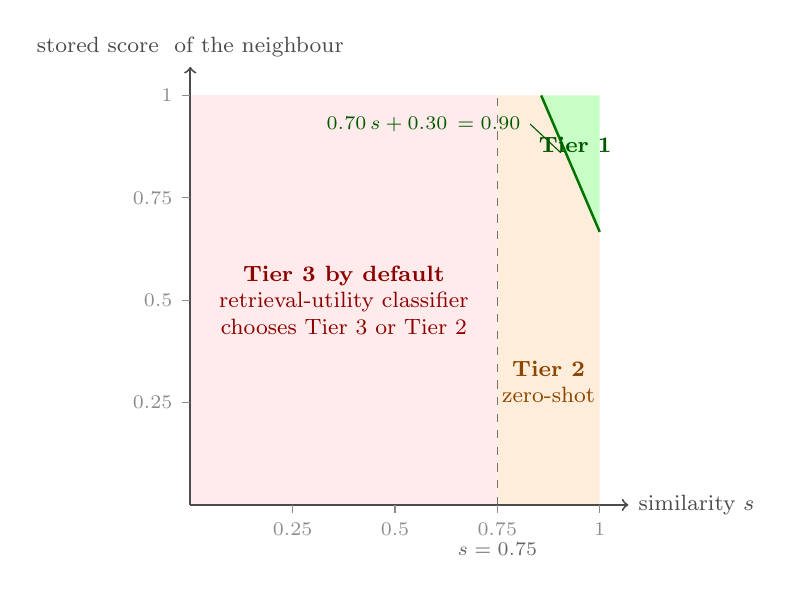
\begin{tikzpicture}[scale=5.2, font=\small]
  \fill[red!8]   (0,0) rectangle (0.75,1);
  \fill[orange!14] (0.75,0) -- (1,0) -- (1,0.6667) -- (0.857,1) -- (0.75,1) -- cycle;
  \fill[green!22] (0.857,1) -- (1,1) -- (1,0.6667) -- cycle;
  \draw[dashed, black!55, line width=0.6pt] (0.75,0) -- (0.75,1);
  \draw[green!45!black, line width=0.9pt] (0.857,1) -- (1,0.6667);
  \draw[->, black!70, line width=0.7pt] (0,0) -- (1.07,0) node[right, font=\footnotesize] {similarity $s$};
  \draw[->, black!70, line width=0.7pt] (0,0) -- (0,1.07) node[above, font=\footnotesize] {stored score $\ustored$ of the neighbour};
  \foreach \x in {0.25,0.5,0.75,1} \draw[black!45] (\x,0) -- (\x,-0.02) node[below, font=\scriptsize] {\x};
  \foreach \y in {0.25,0.5,0.75,1} \draw[black!45] (0,\y) -- (-0.02,\y) node[left, font=\scriptsize] {\y};
  \node[align=center, text=red!55!black, font=\footnotesize] at (0.375,0.5) {\textbf{Tier 3 by default}\\retrieval-utility classifier\\chooses Tier 3 or Tier 2};
  \node[align=center, text=orange!55!black, font=\footnotesize] at (0.875,0.3) {\textbf{Tier 2}\\zero-shot};
  \node[text=green!35!black, font=\footnotesize\bfseries] at (0.94,0.88) {Tier 1};
  \node[anchor=east, font=\scriptsize, text=green!35!black] at (0.83,0.93) {$0.70\,s + 0.30\,\ustored = 0.90$};
  \draw[green!35!black, line width=0.4pt] (0.83,0.93) -- (0.905,0.86);
  \node[anchor=north, font=\scriptsize, text=black!60] at (0.75,-0.07) {$s = 0.75$};
\end{tikzpicture}
\caption[Routing map of the three-tier router.]{Routing map of the three-tier router. Before this map is consulted, the safety override sends any query with $\upre < 0.38$ to the retrieval-utility classifier.}
\label{fig:routing-map}
\end{figure}



\begin{algorithm}[!htbp]
\caption[Three-tier router with safety override (Stage~3).]{Three-tier router with safety override (Stage~3).}
\label{alg:router}
\begin{algorithmic}[1]
\Require similarity $s$, neighbour score $\ustored$, pre-routing confidence $\upre$
\Require $\lambda = 0.70$, $\theta_{1} = 0.90$, $\theta_{\text{sim}} = 0.75$, per-benchmark floor $\phi_{\text{safe}}$ ($0.38$ unless refitted)
\State $\mathcal{S} \gets \lambda\, s + (1-\lambda)\, \ustored$
\If{$\upre < \phi_{\text{safe}}$}
    \State \Return Tier 3 \Comment{safety override; refined by \Cref{alg:ruc}}
\ElsIf{$\mathcal{S} \ge \theta_{1}$}
    \State \Return Tier 1
\ElsIf{$s \ge \theta_{\text{sim}}$}
    \State \Return Tier 2
\Else
    \State \Return Tier 3 \Comment{fall-through; refined by \Cref{alg:ruc}}
\EndIf
\end{algorithmic}
\end{algorithm}

\subsection{Retrieval-utility classifier}
\label{sec:ruc}

Retrieval does not help every question. On questions built around a popular misconception, retrieved passages can reinforce the misconception, and on questions the generator already knows they can distract it. An earlier trajectory without a routing refinement showed this: TruthfulQA exact match fell from cycle to cycle as retrieval-amplified answers entered the verified pool. The selective-retrieval literature reached the same conclusion, including Mallen et al.~\cite{mallen2023whennot}, Wang et al.~\cite{wang2023skr}, Jeong et al.~\cite{jeong2024adaptive} and Baek et al.~\cite{baek2025probing} (\Cref{sec:lit-selective-retrieval}). The retrieval-utility classifier is CAEM's response: whenever the router would send a query to retrieval by default, the classifier predicts whether retrieval will help and, if not, sends the query to Tier 2 instead (\Cref{tab:ruc-dispatch}, \Cref{alg:ruc}).

\textbf{Model:} a logistic regression on $36$ standardised features outputs $p_{\text{RAG}}$, the probability that retrieval helps. The query goes to Tier 3 if $p_{\text{RAG}} \ge 0.375$ and to Tier 2 otherwise. The threshold is below $0.5$ because it was chosen to maximise the number of correctly routed queries of both kinds on held-out folds, and missing a question that needed retrieval was the more common error.

\textbf{Features:} three groups. (i) Question surface: length, the interrogative word, negation, temporal and numerical cues, entity count, a misconception-phrasing pattern, and three style markers (adversarial, opinion-seeking, open-ended). (ii) The top retrieved passage: its similarity, entity overlap with the question, whether the question expects a year or number and whether the passage contains one, and whether the question's main entity appears in Wikidata. (iii) Retrieval quality and self-knowledge: statistics of the top-five retrieval similarities, of their cross-encoder rerank scores and of pairwise entailment among them, plus a self-knowledge probe $p_{\text{IK}}$ in the style of Kadavath et al.~\cite{kadavath2022language}, which reads the base generator's last hidden state and predicts whether it knows the answer without retrieval. The probe was trained on $11{,}980$ questions (out-of-fold AUROC $0.771$). It carries the largest weight in the classifier ($-1.77$): when the generator knows the answer, the classifier leans strongly toward Tier 2. Six features (page views and the four year and number features of the passage) were constant in the training data and received zero weight, and the top-passage similarity took the opposite sign to the one expected.

\textbf{Training data:} $3{,}208$ questions from a pool disjoint from every other fold, drawn from eight benchmarks (the five of the evaluation panel plus Natural Questions, HaluEval-QA and OpenBookQA, included only to widen the range of cases). Each question was answered both with and without retrieval by the same backbone. It was labelled \emph{retrieval helps} ($1{,}846$ questions) if only the retrieval answer was correct and \emph{retrieval hurts} ($1{,}362$) if only the zero-shot answer was correct; questions where both or neither were correct were dropped, because there the routing choice does not matter. TruthfulQA answers were judged by the language-model judge used throughout the thesis. The three extra benchmarks feed nothing else in the architecture.

\textbf{Fitting and accuracy:} nested five-fold stratified cross-validation chose the regularisation strength ($C = 0.5$) in the inner folds and measured accuracy in the outer folds. The pooled out-of-fold AUROC is $0.850$ (standard deviation across folds $0.008$). At the chosen threshold the classifier routes $77.2$ percent of held-out questions correctly ($2{,}477$ of $3{,}208$): $1{,}554$ of $1{,}846$ retrieval-helps questions (recall $0.842$) and $923$ of $1{,}362$ retrieval-hurts questions (specificity $0.678$). Per-benchmark AUROC on the evaluation panel is FEVER $0.718$, TriviaQA $0.936$, CommonsenseQA $0.728$, TruthfulQA $0.732$ and StrategyQA $0.852$ (the last on only $43$ questions). TruthfulQA, the benchmark that motivated the classifier, falls just short of the $0.75$ target set for it in advance.

\textbf{Frozen at deployment:} the classifier was fitted once before the main run and never refitted. Its inputs come from parts of the system that do not change across cycles (the question, the passage index, the base generator with the adapter disabled, and the fixed reranker), so a frozen classifier keeps its routing auditable. This light, classifier-only design agrees with Marina et al.~\cite{moskvoretskii2025llm}, who find that an external classifier matches language-model-based selective retrievers; CAEM differs in reusing the reranker and entailment judge that the verifier already loads. The effect of the classifier is measured in \Cref{sec:ruc-ablation}.

\begin{table}[!htbp]
\centering
\small
\begin{tabular}{@{}p{1.2cm}p{1.3cm}>{\raggedright\arraybackslash}p{5.7cm}>{\raggedright\arraybackslash}p{4.2cm}@{}}
\toprule
\textbf{Order} & \textbf{Tier} & \textbf{Condition} & \textbf{Output path} \\
\midrule
1 & Tier 3 / 2 & $\upre < 0.38$ (safety override): Tier 3 if $p_{\text{RAG}} \ge 0.375$, else Tier 2 & Retrieval-augmented or zero-shot generation \\
2 & Tier 1 & $\mathcal{S} = 0.7\,s + 0.3\,\ustored \ge 0.90$ & Serve neighbour's stored answer \\
3 & Tier 2 & $s \ge 0.75$ & Zero-shot generation \\
4 & Tier 3 / 2 & otherwise (fall-through): Tier 3 if $p_{\text{RAG}} \ge 0.375$, else Tier 2 & Retrieval-augmented or zero-shot generation \\
\bottomrule
\end{tabular}
\caption[Dispatch rules of the router and the retrieval-utility classifier.]{Dispatch rules of the router and the retrieval-utility classifier, in order of evaluation. The classifier is consulted only in rows 1 and 4, the two cases that would otherwise always retrieve.}
\label{tab:dispatch-rules}
\label{tab:ruc-dispatch}
\end{table}

\begin{algorithm}[!htbp]
\caption[Retrieval-utility classifier (Stage~3b).]{Retrieval-utility classifier (Stage~3b).}
\label{alg:ruc}
\begin{algorithmic}[1]
\Require question $q$, router decision $d \in \{\text{Tier 1}, \text{Tier 2}, \text{Tier 3}\}$, frozen scaler $\Sigma$, frozen weights $w$, threshold $\tau_{\text{RUC}} = 0.375$
\If{$d \in \{\text{Tier 1}, \text{Tier 2}\}$}
    \State \Return $d$ \Comment{the classifier does not gate these outcomes}
\EndIf
\State $\mathbf{x} \gets$ [question-surface features, top-passage features, retrieval-quality features, $p_{\text{IK}}$]
\State $p_{\text{RAG}} \gets \sigma\!\left(w^{\top}\, \Sigma(\mathbf{x})\right)$
\State \Return Tier 3 \textbf{if} $p_{\text{RAG}} \ge \tau_{\text{RUC}}$ \textbf{else} Tier 2
\end{algorithmic}
\end{algorithm}

\subsection{Verifier ensemble}
\label{sec:verifier}

The verifier turns a generated answer into nine signals in four families (\Cref{tab:verifier-signals}, \Cref{fig:verifier-flow}, \Cref{alg:verifier}). The families follow the confidence-estimation survey of Geng et al.~\cite{geng2024survey}, with one addition, a separate relevance family, for answers that are supported by a passage but do not address the question. Each family reads a different source of evidence, so that one failure mode does not hide behind another. Two practical details matter. First, the grounding signals check the answer rewritten as a statement: a FEVER \emph{refutes} answer is checked as the negated claim, and a multiple-choice letter is replaced by the text of the chosen option. Second, five shared computations produce all nine signals, so the cost is paid once per answer.

% Verifier data flow (Stage 5): three shared computations feed the nine signals.
\begin{figure}[!htbp]
\centering
\resizebox{\textwidth}{!}{%
\begin{tikzpicture}[
  font=\small,
  inp/.style={rectangle, rounded corners=2pt, draw=black!55, fill=black!4, line width=0.9pt, align=center, inner sep=5pt, text width=2.4cm},
  gen/.style={rectangle, rounded corners=4pt, draw=teal!65!black, fill=teal!8, line width=0.9pt, align=center, inner sep=3pt, text width=4.6cm, font=\footnotesize},
  sig/.style={rectangle, rounded corners=3pt, line width=0.8pt, align=center, inner sep=3pt, text width=3.0cm, font=\footnotesize, minimum height=0.62cm},
  flow/.style={-{Stealth[length=2.2mm]}, line width=0.8pt, draw=black!65},
]
  \node[inp] (qa) at (0,0) {question $+$\\served answer};
  \node[gen] (tf)   at (4.6,3.2) {\textbf{teacher-forced pass}\\{\footnotesize probability of the answer's tokens}};
  \node[gen] (drop) at (4.6,1.6) {\textbf{$K{=}5$ samples, dropout on}\\{\footnotesize do they reach the same answer?}};
  \node[gen] (ch)   at (4.6,0.0) {\textbf{$M{=}3$ sampled chains}\\{\footnotesize temperature $0.7$}};
  \node[gen] (ret)  at (4.6,-1.6) {\textbf{retrieve $20$, rerank to $3$}\\{\footnotesize Wikipedia passages}};
  \node[gen] (ce)   at (4.6,-3.2) {\textbf{cross-encoder}\\{\footnotesize question against answer}};
  \node[sig, draw=blue!60!black, fill=blue!6]   (utok) at (9.6,3.2) {$u_{\text{token}}$};
  \node[sig, draw=blue!60!black, fill=blue!6]   (udro) at (9.6,1.6) {$u_{\text{dropout}}$, then $u_{\text{internal}}$};
  \node[sig, draw=violet!60!black, fill=violet!6] (sa)  at (9.6,0.0) {$s_{\text{avg}}$,\ $p_{\text{entail}}$};
  \node[sig, draw=green!50!black, fill=green!7] (pg)   at (9.6,-1.6) {$p_{\text{ground,max}}$, $p_{\text{ground,mean}}$, $p_{\text{ground,atomic}}$};
  \node[sig, draw=orange!70!black, fill=orange!8] (qar) at (9.6,-3.2) {$q_{\text{match}}$};
  \node[inp, text width=2.3cm] (out) at (13.4,0) {nine signals\\to the calibrated composite};
  \foreach \g in {tf,drop,ch,ret,ce} \draw[flow] (qa.east) -- (\g.west);
  \draw[flow] (tf) -- (utok); \draw[flow] (drop) -- (udro); \draw[flow] (ch) -- (sa); \draw[flow] (ret) -- (pg); \draw[flow] (ce) -- (qar);
  \foreach \s in {utok,udro,sa,pg,qar} \draw[flow] (\s.east) -- (out.west);
  \node[font=\scriptsize, text=black!60, align=left, anchor=north west] at (6.6,-3.9) {colours: internal calibration (blue), sample-set agreement (violet),\\external grounding (green), question--answer match (orange)};
\end{tikzpicture}}
\caption[Where the nine verifier signals come from.]{Where the nine verifier signals come from. Five shared computations produce all nine signals; the grounding scores check the answer rewritten as a statement against the reranked passages.}
\label{fig:verifier-flow}
\end{figure}


\begin{table}[!htbp]
\centering
\footnotesize
\begin{tabular}{@{}>{\raggedright\arraybackslash}p{2.0cm}>{\raggedright\arraybackslash}p{2.2cm}>{\raggedright\arraybackslash}p{5.2cm}>{\raggedright\arraybackslash}p{4.0cm}@{}}
\toprule
\textbf{Signal} & \textbf{Family} & \textbf{What it measures} & \textbf{Failure it catches} \\
\midrule
$u_{\text{token}}$ & Internal & Geometric mean probability of the answer's tokens under the generator & Low-confidence generation \\
$u_{\text{dropout}}$ & Internal & Share of $5$ dropout-active samples whose answer differs from the most common one & Unstable answers \\
$u_{\text{internal}}$ & Internal & $0.5\,u_{\text{token}} + 0.5\,(1-u_{\text{dropout}})$ & Summary of internal confidence \\
$s_{\text{avg}}$ & Sample-set & Mean pairwise cosine similarity of $3$ sampled chains (temperature $0.7$) & Disagreement across chains \\
$p_{\text{entail}}$ & Sample-set & Mean entailment of the answer by each of the $3$ chains & Answer not supported by the model's own reasoning \\
$p_{\text{ground,max}}$ & Grounding & Entailment of the answer by the best of the top three reranked passages & No supporting passage \\
$p_{\text{ground,mean}}$ & Grounding & Mean entailment over the top three passages & Weak overall support \\
$p_{\text{ground,atomic}}$ & Grounding & Weakest support among the answer's atomic facts (answers of $12$ tokens or more) & One fabricated detail in a long answer \\
$q_{\text{a,rel}}$ & Relevance & Cross-encoder relevance of the answer to the question & Off-topic answer \\
\bottomrule
\end{tabular}
\caption[The nine verifier signals.]{The nine verifier signals, grouped by family.}
\label{tab:verifier-signals}
\end{table}

\begin{algorithm}[!htbp]
\caption[Verifier ensemble (Stage~5).]{Verifier ensemble (Stage~5).}
\label{alg:verifier}
\begin{algorithmic}[1]
\Require question $q$, answer $a$, generator $G$, entailment judge $J$, cross-encoder $X$
\Statex \textbf{Internal calibration}
\State $u_{\text{token}} \gets$ geometric mean probability of the tokens of $a$ under $G$ (teacher-forced)
\State draw $5$ answers from $G$ with dropout active; $u_{\text{dropout}} \gets 1 - (\text{count of the most common answer})/5$
\State $u_{\text{internal}} \gets 0.5\,u_{\text{token}} + 0.5\,(1-u_{\text{dropout}})$
\Statex \textbf{Sample-set agreement}
\State $c_{1}, c_{2}, c_{3} \gets$ chains sampled from $G$ at temperature $0.7$
\State $s_{\text{avg}} \gets$ mean pairwise cosine similarity of the chain embeddings
\State $p_{\text{entail}} \gets \tfrac{1}{3}\sum_{m} J(c_{m} \to a)$
\Statex \textbf{External grounding}
\State $P_{1}, P_{2}, P_{3} \gets$ top $3$ of the $20$ retrieved passages after reranking by $X$
\State $h \gets$ $a$ rewritten as a statement \Comment{negated claim for \emph{refutes}; option text for a letter}
\State $p_{\text{ground,max}} \gets \max_{k} J(P_{k} \to h)$; \quad $p_{\text{ground,mean}} \gets \mathrm{mean}_{k}\, J(P_{k} \to h)$
\If{$a$ has at least $12$ tokens and yields atomic facts $f_{1}, \dots, f_{r}$}
    \State $p_{\text{ground,atomic}} \gets \min_{i} \max_{k} J(P_{k} \to f_{i})$
\Else
    \State $p_{\text{ground,atomic}} \gets p_{\text{ground,mean}}$
\EndIf
\Statex \textbf{Relevance}
\State $q_{\text{a,rel}} \gets X(q, a)$
\State \Return the nine signals
\end{algorithmic}
\end{algorithm}

\subsubsection{Internal calibration signals}
\label{sec:verifier-internal}

These signals read the generator's own state. The token signal is the most local form of self-doubt. The dropout signal follows the Bayesian reading of dropout of Gal and Ghahramani~\cite{pmlr-v48-gal16}: with dropout switched on, the generator draws five answers, and $u_{\text{dropout}}$ is the share that disagree with the most common one, so $0$ means all five agree. The summary $u_{\text{internal}}$ is the input to the confabulation early-exit rule (\Cref{sec:decision}), because it isolates internal confidence from external evidence. This family is the one most affected by fine-tuning, which is one reason stored entries are re-verified at every cycle boundary. A hidden-state eigenvalue score \cite{chen2024inside} was considered as a replacement for the dropout signal but not adopted, for cost.

\subsubsection{Sample-set agreement signals}
\label{sec:verifier-sample-set}

These signals ask whether the generator gives the same answer when it reasons again. The generator samples three chains; $s_{\text{avg}}$ is their mean pairwise similarity in the embedding space, an embedding-based form of the self-consistency of Wang et al.~\cite{wang2023selfconsistency}, and $p_{\text{entail}}$ asks the judge whether each chain supports the served answer. Both use the same three chains.

Two dispersion signals were dropped before the main run. The semantic entropy of Farquhar et al.~\cite{farquhar2024semantic} (after Kuhn et al.~\cite{kuhn2023semantic}), computed over $10$ samples at temperature $1.0$, received a learned weight of about $-0.0005$ in the ten-signal cycle-zero fit, so it added nothing beyond the two signals above, while its $10$ samples were the largest single cost of the verifier. The kernel language entropy of Nikitin et al.~\cite{nikitin2024kle} needs the same samples and was not adopted either.

\subsubsection{External grounding signals}
\label{sec:verifier-grounding}

These signals check the answer, rewritten as a statement, against the three best passages. The maximum catches the case where one passage clearly supports the answer; the mean rewards support spread over several passages; the atomic score splits a long answer into atomic facts, in the FActScore manner of Min et al.~\cite{min-etal-2023-factscore}, and takes the weakest-supported fact, so that one fabricated detail is not averaged away. The atomic score applies only to answers of at least $12$ tokens and otherwise equals the mean score.

\textbf{Realised run:} in the main run the atomic score equalled the mean score on all $14{,}951$ scored samples. The length gate skipped $99.0$ percent of answers, and for the remaining $1.0$ percent the decomposer returned no atomic facts. This is a mismatch of scope rather than a tuning fault: the signal follows FActScore, which targets long-form text, while the answers on this panel are labels, option letters and short entities, each already a single fact, so a lower gate would only reproduce the mean score. The signal is part of the design but contributed no separate information in this run; applying the same check to the reasoning chain, where several facts are asserted, is left as future work (\Cref{ch:conclusion}).

\subsubsection{Question-answer relevance}
\label{sec:verifier-qa-rel}

The relevance signal scores the answer against the question with the cross-encoder. It forms its own family because an off-topic answer can be fully supported by a passage that is itself off-topic, which the grounding signals cannot detect. In the cycle-zero composite it received the largest weight of the nine signals ($0.491$, \Cref{sec:composite-boost}).

\subsection{Calibrated probability composite}
\label{sec:composite}

The composite turns the nine signals into one probability of correctness, $\ustored$, in three steps (\Cref{fig:composite-pipeline}, \Cref{alg:composite}).
\begin{enumerate}
    \item \textbf{One curve per signal:} isotonic regression maps each raw signal to the probability that the answer is correct.
    \item \textbf{Per benchmark, with shrinkage:} the curves are also fitted on each training benchmark and pulled part of the way toward the pooled curve, so that benchmarks with little data do not overfit.
    \item \textbf{Weighted sum:} a regularised logistic regression combines the nine calibrated probabilities, in log-odds, into $\ustored$.
\end{enumerate}
All three steps are fitted on the calibration fold ($500$ labelled questions from each training benchmark) and refitted at every cycle boundary on the same fold re-scored with the new adapter.

% Calibrated probability composite (Stage 5 to 6).
\begin{figure}[!htbp]
\centering
\resizebox{\textwidth}{!}{%
\begin{tikzpicture}[
  font=\small,
  box/.style={rectangle, rounded corners=4pt, line width=0.9pt, align=center, inner sep=5pt, text width=3.1cm, minimum height=1.55cm},
  flow/.style={-{Stealth[length=2.2mm]}, line width=0.9pt, draw=black!65},
]
  \node[box, draw=black!55, fill=black!4, text width=2.2cm] (s) at (0,0) {\textbf{nine raw}\\\textbf{signals}};
  \node[box, draw=blue!60!black, fill=blue!6] (iso) at (3.6,0) {\textbf{1. one curve per signal}\\{\footnotesize raw value $\to$ probability the answer is correct (isotonic)}};
  \node[box, draw=violet!60!black, fill=violet!6] (shr) at (7.7,0) {\textbf{2. per benchmark}\\{\footnotesize each benchmark's curve pulled $40\%$ toward the pooled curve}};
  \node[box, draw=green!50!black, fill=green!7] (bst) at (11.8,0) {\textbf{3. weighted sum}\\{\footnotesize log-odds combined by a regularised logistic regression}};
  \node[box, draw=orange!70!black, fill=orange!8, text width=1.9cm] (u) at (15.2,0) {$\ustored$\\{\footnotesize one probability}};
  \draw[flow] (s) -- (iso); \draw[flow] (iso) -- (shr); \draw[flow] (shr) -- (bst); \draw[flow] (bst) -- (u);
\end{tikzpicture}}
\caption[The calibrated probability composite in three steps.]{The calibrated probability composite in three steps. All three are refitted at every cycle boundary on the re-scored calibration fold.}
\label{fig:composite-pipeline}
\end{figure}


\begin{algorithm}[!htbp]
\caption[Calibrated probability composite (fit and predict).]{Calibrated probability composite (fit and predict).}
\label{alg:composite}
\begin{algorithmic}[1]
\Statex \textbf{Fit stage:} calibration fold split by benchmark, $\mathcal{D}_{b}$ for $b \in \mathcal{B}$, each a set of signal vectors $x \in \mathbb{R}^{9}$ with exact-match labels $y \in \{0,1\}$; pooled fold $\mathcal{D} = \bigcup_{b}\mathcal{D}_{b}$.
\For{each signal $j$}
    \State direction $\gets$ sign of the Pearson correlation of $x_{j}$ with $y$ on $\mathcal{D}$
    \State fit an isotonic curve $\mathrm{iso}_{j}$ in that direction on $\mathcal{D}$, with outputs clipped to $[0.02, 0.98]$
\EndFor
\For{each benchmark $b$ and signal $j$}
    \State fit $\mathrm{iso}^{b}_{j}$ on $\mathcal{D}_{b}$; at each knot $x$ set $\mathrm{iso}^{b}_{j}(x) \gets 0.6\,\mathrm{iso}^{b}_{j}(x) + 0.4\,\mathrm{iso}_{j}(x)$
\EndFor
\State $L_{ij} \gets \mathrm{logit}\big(\mathrm{iso}_{j}(x_{ij})\big)$ on $\mathcal{D}$; fit logistic regression ($\ell_{2}$ penalty, $C = 0.01$) of $y$ on $L$ to get weights $\mathbf{w}$ and intercept $b_{0}$
\State repeat the logistic fit on each $\mathcal{D}_{b}$ with the shrunk curves to get $(\mathbf{w}_{b}, b_{0,b})$
\Statex \textbf{Predict stage:} signal vector $x$ and benchmark tag $b^{\star}$
\State use the curves and weights of $b^{\star}$ if $b^{\star} \in \mathcal{B}$, otherwise the pooled ones
\State \Return $\ustored \gets \sigma\!\Big(b_{0} + \sum_{j} w_{j}\, \mathrm{logit}\big(\mathrm{iso}_{j}(x_{j})\big)\Big)$
\end{algorithmic}
\end{algorithm}

\subsubsection{Per-signal isotonic regression}
\label{sec:composite-isotonic}

Isotonic regression fits any monotone curve, not only a logistic one, which matters because some signals saturate near the top of their range; and it needs less data than histogram binning because neighbouring bins share information. Niculescu-Mizil and Caruana~\cite{niculescu2005predicting} found isotonic regression the stronger post-hoc calibrator when enough data are available, but prone to overfitting below roughly $200$ to $1{,}000$ calibration points, where Platt scaling does better. The per-benchmark folds here hold $500$ points each, which is one reason the per-benchmark curves are shrunk toward the pooled curve (\Cref{sec:composite-shrinkage}). The direction of each curve is taken from the sign of the signal's correlation with correctness, so a signal where high means unsafe (such as $u_{\text{dropout}}$) needs no special handling. Probabilities are clipped to $[0.02, 0.98]$ so that no single signal can dominate the log-odds sum, and a signal with fewer than $50$ calibration samples is left out.

\subsubsection{Per-benchmark fit with shrinkage prior}
\label{sec:composite-shrinkage}

Each training benchmark gets its own curves, blended at every knot with the pooled curve: $60$ percent benchmark curve, $40$ percent pooled curve, a convex blend in the spirit of James--Stein shrinkage. Each benchmark also gets its own logistic weights. The blend strength was chosen to balance two effects visible in the cycle-zero sweep: on the held-out validation fold, fitting each benchmark more freely ($\alpha_{\text{shrink}}$ closer to $1$) stored more answers but separated correct from incorrect answers less well (pooled Cohen's $d$ of $0.85$ at $\alpha_{\text{shrink}} = 0$, $0.72$ at $0.6$ and $0.66$ at $1$; \Cref{ch:evaluation}). A query from a benchmark outside the training panel uses the pooled curves and weights.

\subsubsection{Boost layer with L2 regularisation}
\label{sec:composite-boost}

The boost layer is a logistic regression on the nine log-odds, following the multi-scoring approach of Valentin et al.~\cite{valentin2024hallucination}. A learned combination is used rather than an equal-weight sum because several signals overlap (the two sample-set signals, and the three grounding signals), and the regression can discount the overlap. An $\ell_{2}$ penalty is used rather than $\ell_{1}$ so that weights shrink smoothly without any signal being dropped, and its strength is strong ($C = 0.01$, chosen in the cycle-zero sweep of \Cref{ch:evaluation}). In the cycle-zero pooled fit every weight is positive; the largest are question-answer relevance ($0.491$), best-passage grounding ($0.379$) and internal confidence ($0.334$).

\subsection{Fixed-threshold storage gate}
\label{sec:conformal-gate}

The storage gate applies two fixed cut-points to $\ustored$: an answer is stored if $\ustored \ge 0.60$ and deferred if $0.45 \le \ustored < 0.60$; below $0.45$, the decision rule of \Cref{sec:decision} chooses between abstaining and discarding. The cut-points were fixed before the main run and never changed.

An earlier design set the cut-points by split-conformal prediction at fixed precision targets and refitted them every cycle. It was replaced because conformal guarantees assume the calibration and evaluation data come from the same distribution, and on this panel they did not: precision on the evaluation fold fell well below the conformal targets, and on the weakest benchmarks the per-benchmark fits rejected almost everything. A fixed cut-point on a calibrated probability, in the spirit of the post-hoc calibration of Niculescu-Mizil and Caruana~\cite{niculescu2005predicting} and the selective classification of Geifman and El-Yaniv~\cite{geifman2017selective}, makes no coverage promise; its precision is simply measured on every fold. It still assumes that calibration and test data are alike, so under distribution shift the realised precision can fall, as Ovadia et al.~\cite{ovadia2019trust} and Kamath et al.~\cite{kamath2020selective} show; TruthfulQA in \Cref{ch:evaluation} is such a case.

\subsubsection{Storage threshold}
\label{sec:conformal-store}

The storage cut-point $\tau_{\text{store}} = 0.60$ was chosen on the cycle-zero calibration fold before the main run, against the stricter alternative $0.65$, which stored about half as many answers (\Cref{ch:evaluation} reports the sweep). The storage class fills the memory and supplies the training pool, so it is guarded on both sides: training requires the stricter $\ustored \ge 0.70$, and the retroactive pass removes entries that later fall below $0.50$.

\subsubsection{Deferral threshold}
\label{sec:conformal-defer}

Answers with $0.45 \le \ustored < 0.60$ go to the deferred buffer, not to memory. They are re-scored at the next cycle boundaries (\Cref{sec:deferred-reconsider}) and either promoted or dropped, so a looser cut-point here costs little: deferred answers never reach the training pool unless they are later promoted. The configuration refuses a deferral cut-point above the storage cut-point.

\subsubsection{Cycle-boundary recalibration}
\label{sec:conformal-cycle-recalib}

The cut-points ($0.60$ and $0.45$), the abstention floor ($0.20$), the retroactive prune threshold ($0.50$) and the training threshold ($0.70$) stay fixed for the whole run. What changes at each cycle boundary is the calibration: after a committed fine-tune, the same calibration fold is re-scored with the new adapter, the pre-routing temperatures and safety floors are refitted, and the composite is refitted. The verifier is then reloaded with the new composite before the retroactive pass, so stored entries are re-scored with curves that match the current adapter. Without this order, entries whose raw signals had shifted after fine-tuning would be read through stale curves and wrongly pruned.

Keeping the cut-points fixed while the composite adapts is what lets Hypothesis~1 (\Cref{sec:hypotheses}) test the verifier rather than a moving operating point. A deployed system would run the same refit; the only difference is that its cycle would end on a calendar or accumulation trigger, with a labelled sample of recent admissions as the calibration fold.

\subsection{Four-outcome storage decision}
\label{sec:decision}

The decision rule maps $\ustored$ and two guard signals to one of four outcomes (\Cref{alg:decision}). Four outcomes are used instead of store-or-discard for two reasons. First, an answer just below the storage cut-point is not the same as one near zero: deferring it lets the next cycle's adapter settle it. Second, \emph{I have nothing reliable to say} is a different situation from \emph{I have an answer but cannot ground it}: abstention makes the first an explicit, user-facing refusal, in the spirit of the abstention framework of Yadkori et al.~\cite{yadkori2024abstention}.

\textbf{Confabulation early exit:} checked first, at query time only. An answer the generator is internally confident about but that no passage supports is discarded:
\begin{equation}
\big(u_{\text{internal}} \ge 0.70\big) \;\wedge\; \big(p_{\text{ground,max}} \le 0.20\big)
\;\Rightarrow\; \textsc{Discard}.
\label{eq:early-exit-rule}
\end{equation}
This catches the most damaging case, a confident answer with no evidence, which the composite alone might score as merely borderline.

\textbf{Thresholds:} otherwise the answer is stored if $\ustored \ge 0.60$ and deferred if $\ustored \ge 0.45$. Below $0.45$, the system abstains when the best passage barely supports the answer ($p_{\text{ground,max}} < 0.20$) and discards otherwise. A discarded answer is not stored; it is still shown to the user, with its probability and a warning that the evidence conflicts. An abstention replaces the answer with an insufficient-evidence message.

\begin{algorithm}[!htbp]
\caption[Four-outcome storage decision (Stage~6).]{Four-outcome storage decision (Stage~6).}
\label{alg:decision}
\begin{algorithmic}[1]
\Require $\ustored$, $u_{\text{internal}}$, $p_{\text{ground,max}}$; cut-points $\tau_{\text{store}} = 0.60$, $\tau_{\text{defer}} = 0.45$; early-exit thresholds $\eta_{u} = 0.70$, $\eta_{g} = 0.20$; abstention floor $\phi_{\text{pg}} = 0.20$
\If{query time \textbf{and} $u_{\text{internal}} \ge \eta_{u}$ \textbf{and} $p_{\text{ground,max}} \le \eta_{g}$}
    \State \Return \textsc{Discard} \Comment{confabulation early exit}
\EndIf
\If{$\ustored \ge \tau_{\text{store}}$} \State \Return \textsc{Store} \EndIf
\If{$\ustored \ge \tau_{\text{defer}}$} \State \Return \textsc{Defer} \EndIf
\If{$p_{\text{ground,max}} < \phi_{\text{pg}}$} \State \Return \textsc{Abstain} \EndIf
\State \Return \textsc{Discard}
\end{algorithmic}
\end{algorithm}

\subsection{Cycle-boundary maintenance}
\label{sec:cycle-boundary}

The cycle-boundary steps are where the two kinds of statelessness of \Cref{sec:arch-opportunity} are addressed. Fine-tuning on verified answers, many produced with retrieval, is meant to let the generator answer later questions of the same kind without retrieval. The memory is meant to serve repeated questions at the cost of a lookup, with re-verification keeping each stored score in line with the current model. The deferred pass gives borderline answers a second chance under the new adapter. The steps run in the order of \Cref{fig:cycle-boundary-order}; on a cycle whose fine-tune is rolled back, all steps after the retention guard are skipped.

\subsubsection{Retroactive re-verification}
\label{sec:retroverify}

The retroactive pass re-scores every stored episode with the current adapter and the refitted composite (\Cref{alg:retroverify}). An entry is removed if its reasoning chain is caught by the repetition filter or if its new $\ustored$ is below $0.50$. Otherwise all nine stored signals and $\ustored$ are overwritten with the new values, which may be lower or higher than before. The prune threshold sits below the deferral cut-point, so an entry that is no longer storage-quality but still plausible is kept rather than discarded. The pass removed $56$, $271$, $352$ and $382$ entries at cycles one, two, three and five (it was skipped at cycle four), that is $13$, $9$, $7$ and $4$ percent of the entries it checked.

\begin{algorithm}[!htbp]
\caption[Retroactive re-verification pass (Stage~8).]{Retroactive re-verification pass (Stage~8).}
\label{alg:retroverify}
\begin{algorithmic}[1]
\Require memory $\mathcal{M}$, verifier with the current adapter and refitted composite, prune threshold $\tau_{\text{retro}} = 0.50$
\For{each entry $e \in \mathcal{M}$}
    \If{the reasoning chain of $e$ is caught by the repetition filter}
        \State remove $e$; \textbf{continue}
    \EndIf
    \State $\mathbf{x} \gets \mathrm{verify}(e.\text{question}, e.\text{answer})$ \Comment{early exit disabled}
    \If{$\mathbf{x}.\ustored < \tau_{\text{retro}}$}
        \State remove $e$
    \Else
        \State overwrite the signals and $\ustored$ of $e$ with $\mathbf{x}$ \Comment{may lower or raise $\ustored$}
    \EndIf
\EndFor
\end{algorithmic}
\end{algorithm}

\subsubsection{Deferred-entry reconsideration}
\label{sec:deferred-reconsider}

Each deferred answer is re-scored at the next cycle boundaries (\Cref{alg:deferred-reconsider}). It is promoted into memory if the verifier now decides to store it ($\ustored \ge 0.60$); it is dropped once it has been reconsidered twice without promotion; otherwise it waits for the next pass. The buffer holds at most $10{,}000$ answers and evicts the oldest when full. The passes promoted $131$, $220$ and $299$ answers at cycles two, three and five; the first pass, at cycle one, found an empty buffer, and the pass was skipped at cycle four. The memory consolidation of \Cref{sec:memory-store} runs straight after this pass.

\begin{algorithm}[!htbp]
\caption[Deferred-entry reconsideration pass (Stage~8).]{Deferred-entry reconsideration pass (Stage~8).}
\label{alg:deferred-reconsider}
\begin{algorithmic}[1]
\Require deferred buffer $\mathcal{B}$, current verifier, $\tau_{\text{store}} = 0.60$, time-to-live $\tau_{\text{ttl}} = 2$ passes
\For{each entry $e \in \mathcal{B}$}
    \State $\mathbf{x} \gets \mathrm{verify}(e)$
    \If{$\mathbf{x}.\text{decision} = \textsc{Store}$ \textbf{and} $\mathbf{x}.\ustored \ge \tau_{\text{store}}$}
        \State move $e$ into the memory
    \ElsIf{$e.\text{age} + 1 \ge \tau_{\text{ttl}}$}
        \State drop $e$
    \Else
        \State $e.\text{age} \gets e.\text{age} + 1$ \Comment{wait for the next pass}
    \EndIf
\EndFor
\end{algorithmic}
\end{algorithm}

\subsubsection{Self-improvement loop}
\label{sec:sil}

The self-improvement loop fine-tunes the generator on its own verified answers. It belongs to the family of methods that train a model on its filtered outputs \cite{NEURIPS2022_639a9a17,hosseini2024vstar,gulcehre2023rest}, and is related to distilling a teacher's filtered reasoning into a student \cite{ho2023large}. Its intended role is to turn verified retrieval-based reasoning into knowledge the generator holds without retrieval. Song et al.~\cite{song2024gap} find that such loops need a positive gap between how well a model generates and how well it can verify, and saturate within a few rounds; Fu et al.~\cite{fu2025collapse} show in linear regression that filtering through an external verifier prevents collapse but pulls the model toward the verifier's own knowledge. CAEM's external verifier and fixed cut-points are meant to keep the training pool above the purification condition of \Cref{thm:bayes-purity}. The loop has five steps (\Cref{alg:sil}).

\textbf{Select:} take stored episodes with $\ustored \ge 0.70$ from the three training benchmarks only, so transfer benchmarks never reach the gradient. The training target is the stored reasoning chain and answer; most chains were written under the retrieval prompt.

\textbf{Rebalance:} reweight the pool so that no benchmark dominates: per-benchmark counts are mixed with a softmax at temperature $2$, upsampling is capped at three times a benchmark's count, each benchmark contributes at least $50$ examples, a benchmark with no verified episodes is given $100$ gold-labelled examples from its training split, and no benchmark exceeds $40$ percent of the pool. This addresses the failure of an earlier run, in which one benchmark grew to the whole training pool.

\textbf{Train:} train a low-rank adapter (LoRA, rank $32$, scaling $64$, dropout $0.05$) on all seven linear projections of every transformer block, following the all-layer recommendation of Biderman et al.~\cite{biderman2024lora}; the backbone stays frozen. Training runs for $3$ epochs with 32-bit AdamW at a learning rate of $2 \times 10^{-4}$, an effective batch of $16$ and gradient checkpointing. The loss is cross-entropy alone:
\begin{equation}
\mathcal{L}(\boldsymbol{\theta}) \;=\; \mathcal{L}_{\mathrm{CE}}(\boldsymbol{\theta}) \;+\; \tfrac{\lambda_{\text{anc}}}{2}\, \big\| \boldsymbol{\theta} - \boldsymbol{\theta}^{(t-1)} \big\|_{2}^{2}, \qquad \lambda_{\text{anc}} = 0,
\label{eq:sil-anchor}
\end{equation}
where $\boldsymbol{\theta}$ are the adapter parameters and $\boldsymbol{\theta}^{(t-1)}$ the previous cycle's adapter. The anchor term, a uniform-weight simplification of the elastic weight consolidation of Kirkpatrick et al.~\cite{doi:10.1073/pnas.1611835114}, belongs to the full fine-tuning path used in an earlier run and is switched off here: the frozen backbone and the small adapter already limit how far each cycle can move the model, and in the earlier run the anchor outweighed the learning signal from the small training pool.

\textbf{Check retention:} before the first cycle, record the accuracy of the untouched model on three held-out probes of $200$ questions each: MMLU (general knowledge), the TriviaQA test fold (open-text facts) and the CommonsenseQA test fold (commonsense multiple choice). After each fine-tune, compute each probe's accuracy as a ratio of that starting value (\Cref{eq:nfr-retention-floor}).

\textbf{Commit or roll back:} keep the new adapter only if every ratio is at least $0.93$; otherwise restore the previous adapter. The memory is kept either way. Requiring every probe, not just the average, to pass is deliberate: an earlier rule that watched only MMLU missed forgetting on narrower tasks. In the main run the guard fired once, at cycle four, when the TriviaQA test ratio fell to $0.886$.

\begin{algorithm}[!htbp]
\caption[Self-improvement loop with retention guard (Stage~8).]{Self-improvement loop with retention guard (Stage~8).}
\label{alg:sil}
\begin{algorithmic}[1]
\Require memory $\mathcal{M}$, previous adapter $\boldsymbol{\theta}^{(t-1)}$, probes $\mathcal{P}$ with starting accuracies $A_{0}^{p}$, $\tau_{\text{train}} = 0.70$, $\rho_{\min} = 0.93$
\State $\mathcal{T} \gets$ rebalance$\big(\{e \in \mathcal{M} : e.\ustored \ge \tau_{\text{train}},\ e \text{ from a training benchmark}\}\big)$
\State $\boldsymbol{\theta}^{\star} \gets$ train the adapter on $\mathcal{T}$ with $\mathcal{L}_{\mathrm{CE}}$, starting from $\boldsymbol{\theta}^{(t-1)}$
\If{$\min_{p \in \mathcal{P}} A^{p}(\boldsymbol{\theta}^{\star}) / A_{0}^{p} \ge \rho_{\min}$}
    \State \Return $\boldsymbol{\theta}^{\star}$ \Comment{commit}
\Else
    \State \Return $\boldsymbol{\theta}^{(t-1)}$ \Comment{roll back; memory kept; later cycle-boundary steps skipped}
\EndIf
\end{algorithmic}
\end{algorithm}

Keeping the memory through a rollback is what makes the loop safe to repeat: a failed cycle costs its fine-tuning time but not the answers it verified. This asymmetry underlies the memory part of \Cref{cor:stochastic-equilibrium}.

\section{Theoretical analysis}
\label{sec:theory}

This section states what can be said formally about the stored pool, and is explicit about the strength of each statement (\Cref{fig:theory-map}). Only two results are proven: a floor on the purity of the stored pool (\Cref{thm:purity}) and the condition under which filtering makes the pool purer than the generator's raw output (\Cref{thm:bayes-purity}). Four remarks are exact calculations on simplified models; they show what the design aims at, not what the system guarantees. Five heuristics describe how the pool is expected to evolve across cycles; they rest on assumptions the real system does not fully meet, so they come with argument sketches rather than proofs, and the evaluation checks them only for consistency.

All statements are about the stored pool. None bounds the accuracy of the fine-tuned generator on new questions, so a fall in held-out accuracy is outside their scope rather than a contradiction of them.

% Status map of the formal statements in sec:theory.
\begin{figure}[!htbp]
\centering
\resizebox{\textwidth}{!}{%
\begin{tikzpicture}[
  font=\small,
  base/.style={rectangle, rounded corners=4pt, align=center, inner sep=4pt, text width=4.4cm, minimum height=1.15cm},
  pr/.style={base, line width=1.1pt, draw=green!45!black, fill=green!10},
  rm/.style={base, line width=0.9pt, draw=blue!55!black, fill=blue!6},
  he/.style={base, line width=0.9pt, dashed, draw=orange!70!black, fill=orange!7},
  dep/.style={-{Stealth[length=2mm]}, line width=0.7pt, draw=black!55},
]
  \node[pr] (purity) at (0,0)     {\textbf{Pool purity floor}\\{\footnotesize \Cref{thm:purity}}};
  \node[pr] (bayes)  at (0,-5.7)  {\textbf{Purification condition}\\{\footnotesize \Cref{thm:bayes-purity}; H1}};
  \node[he] (t1)   at (5.8,1.0)   {\textbf{Tier 1 error ceiling}\\{\footnotesize \Cref{cor:tier1-floor}}};
  \node[rm] (dec)  at (5.8,-0.9)  {\textbf{Error decomposition}\\{\footnotesize \Cref{thm:asymptotic-elim}; H4}};
  \node[rm] (mono) at (5.8,-3.8)  {\textbf{Purity rises with accuracy}\\{\footnotesize \Cref{thm:monotone-purification}}};
  \node[rm] (fix)  at (5.8,-5.7)  {\textbf{Repeated filtering gives purity 1}\\{\footnotesize \Cref{thm:bayes-convergence}; H2}};
  \node[he] (sc)   at (5.8,-7.6)  {\textbf{Self-correction}\\{\footnotesize \Cref{cor:self-correction}}};
  \node[rm] (corp) at (11.6,-0.9) {\textbf{Corpus ceiling}\\{\footnotesize \Cref{cor:corpus-floor}}};
  \node[he] (rate) at (11.6,-3.0) {\textbf{Storage-rate sensitivity}\\{\footnotesize \Cref{thm:monotone}}};
  \node[he] (conv) at (11.6,-4.9) {\textbf{Convergence envelope}\\{\footnotesize \Cref{thm:convergence}; H3}};
  \node[he] (eq)   at (11.6,-6.8) {\textbf{Equilibrium under rollback}\\{\footnotesize \Cref{cor:stochastic-equilibrium}}};
  \draw[dep] (purity.east) -- (t1.west);
  \draw[dep] (purity.east) -- (dec.west);
  \draw[dep] (dec.east) -- (corp.west);
  \draw[dep] (bayes.east) -- (mono.west);
  \draw[dep] (bayes.east) -- (fix.west);
  \draw[dep] (bayes.east) -- (sc.west);
  \draw[dep] (purity.north) |- (8.7,2.3) |- (conv.west);
  \draw[dep] (rate.south) -- (conv.north);
  \draw[dep] (conv.south) -- (eq.north);
  \node[pr, text width=3.4cm, minimum height=0.55cm, font=\footnotesize] at (0,-9.4) {proven};
  \node[rm, text width=3.4cm, minimum height=0.55cm, font=\footnotesize] at (5.8,-9.4) {remark: exact maths on a simplified model};
  \node[he, text width=3.4cm, minimum height=0.55cm, font=\footnotesize] at (11.6,-9.4) {heuristic: argument sketch};
\end{tikzpicture}}
\caption[Status of the formal statements and the hypotheses they inform.]{Status of the formal statements and the hypotheses (H1 to H4) they inform. Arrows point from a statement to those that build on it.}
\label{fig:theory-map}
\end{figure}


\paragraph{The observed horizon:} the main run produced six cycles (zero to five) and stopped after cycle five, as planned after the cycle-four rollback. The automatic early-stop check fired at the same point, but its storage and retention inputs were wired to the wrong quantities, so its firing is not evidence that the trajectory had levelled off (\Cref{sec:env-cycles}). Statements about long-run behaviour are therefore read against these six cycles, which are too few to estimate limits or rates.

\subsection{Pool purity}
\label{sec:theorem-purity}

The \emph{purity} of the stored pool is the share of stored answers that are correct. At each cycle boundary the pool is made of two parts: older entries that survived re-verification, and new entries admitted by the gate during the cycle.

\begin{theorem}[Pool purity floor]
\label{thm:purity}
Let $\pi_{t+1}$ be the expected purity of the stored pool at the end of cycle $t+1$. Assume:
\begin{enumerate}[label=(\roman*)]
    \item \textbf{Fixed gate:} new answers are stored when $\ustored \ge \tau_{\text{store}}$, with $\tau_{\text{store}}$ fixed across cycles.
    \item \textbf{Like calibration data:} the cycle's candidate answers come from the same distribution as the calibration fold, so the expected purity of the new entries equals $\pi_{\text{store}}$, the share of correct answers among calibration-fold answers with $\ustored \ge \tau_{\text{store}}$.
    \item \textbf{Survivors:} the older entries that survive re-verification (score at least $\tau_{\text{retro}}$) have expected purity $\pi_{\text{retro}}$.
\end{enumerate}
Then
\begin{equation}
\pi_{t+1} \;\ge\; \min\!\big(\pi_{\text{store}},\,\pi_{\text{retro}}\big).
\label{eq:thm-purity}
\end{equation}
\end{theorem}

\begin{proof}
Let the pool contain $n_{\text{new}}$ new entries and $n_{\text{old}}$ surviving older entries. Its expected purity is the weighted average
\[
\pi_{t+1} \;=\; \frac{n_{\text{new}}\,\pi_{\text{store}} + n_{\text{old}}\,\pi_{\text{retro}}}{n_{\text{new}} + n_{\text{old}}},
\]
using (i) and (ii) for the new entries (because the cut-point is the same in every cycle, the calibration-fold precision at that cut-point applies to each cycle's admissions) and (iii) for the survivors. A weighted average of two numbers is never smaller than the smaller of them, which gives \Cref{eq:thm-purity}.
\end{proof}

\paragraph{In plain terms:} a mixture of two groups is at least as clean as the dirtier group. The result is simple; its value is that both inputs can be measured. Because the gate never changes (assumption (i)), the calibration-fold precision $\pi_{\text{store}}$ can be read at every cycle, and the precision of the new entries can be checked directly on the stream chunk, whose answers are labelled. The floor holds in expectation, up to the sampling error of the calibration estimate, and only as far as assumption (ii) holds; for a benchmark whose questions differ from the calibration fold, it says nothing.

\paragraph{What the run shows:} on the training panel, the calibration-fold precision at the cut-point was between $0.732$ and $0.746$ in cycles one to five, and the precision of the answers actually stored from each stream chunk was $0.753$, $0.751$, $0.724$, $0.738$ and $0.724$, within about one point of it; assumption (ii) approximately held on the training panel. It did not hold on the transfer benchmark TruthfulQA, where the answers the gate stored on the evaluation fold were correct only $31$ to $38$ percent of the time at cycles one to five (\Cref{tab:decision-matrix-trajectory}). Per-cycle readings are in \Cref{tab:pi-store-trajectory}.

\subsection{When filtering helps: the purification condition}
\label{sec:theorem-bayes}

The floor says how pure the pool is relative to the calibration fold. The next result says when the gate makes the pool purer than the generator's unfiltered answers at all.

\begin{proposition}[Purification condition]
\label{thm:bayes-purity}
Let $p_c \in (0,1)$ be the share of the generator's answers that are correct at cycle $c$, and let $\mathrm{TPR}_c$ and $\mathrm{FPR}_c$ be the shares of correct and of incorrect answers that the gate stores. The purity of the stored answers is
\begin{equation}
P_c \;=\; \frac{p_c \, \mathrm{TPR}_c}{p_c \, \mathrm{TPR}_c \;+\; (1-p_c) \, \mathrm{FPR}_c},
\label{eq:bayes-purity}
\end{equation}
and $P_c > p_c$ if and only if $\mathrm{TPR}_c > \mathrm{FPR}_c$, which is the same as the gate's balanced accuracy $\alpha_c = (\mathrm{TPR}_c + 1 - \mathrm{FPR}_c)/2$ exceeding one half. If the gate errs equally on both classes ($\mathrm{TPR}_c = 1-\mathrm{FPR}_c = \alpha_c$), then $P_c = p_c \alpha_c / \big(p_c \alpha_c + (1-p_c)(1-\alpha_c)\big)$.
\end{proposition}

\begin{proof}
Let $Y \in \{0,1\}$ mark a correct answer and $S \in \{0,1\}$ a stored one, so $\Pr(Y=1) = p_c$, $\Pr(S=1 \mid Y=1) = \mathrm{TPR}_c$ and $\Pr(S=1 \mid Y=0) = \mathrm{FPR}_c$. Bayes' rule gives $P_c = \Pr(Y=1 \mid S=1)$ as in \Cref{eq:bayes-purity}. Then $P_c > p_c$ means $\mathrm{TPR}_c > p_c \mathrm{TPR}_c + (1-p_c)\mathrm{FPR}_c$, that is $(1-p_c)\mathrm{TPR}_c > (1-p_c)\mathrm{FPR}_c$, which for $p_c < 1$ is $\mathrm{TPR}_c > \mathrm{FPR}_c$. Finally $\alpha_c > 1/2$ means $\mathrm{TPR}_c + 1 - \mathrm{FPR}_c > 1$, again $\mathrm{TPR}_c > \mathrm{FPR}_c$.
\end{proof}

\paragraph{In plain terms:} storing purifies only if the gate accepts correct answers more often than wrong ones. A gate that is only a little better than chance still helps, and a gate worse than chance makes the pool dirtier than the generator (\Cref{fig:purity-curves}). This is why the verifier's balanced accuracy is the precondition tested by Hypothesis~1. In the language of learning with noisy labels, the condition is the class-conditional noise condition $\rho_{+} + \rho_{-} < 1$ of Natarajan et al.~\cite{natarajan2013learning}, with $\rho_{+} = 1-\mathrm{TPR}_c$ and $\rho_{-} = \mathrm{FPR}_c$; their learning guarantees also need a noise-corrected loss, which CAEM does not use, so only the condition is borrowed. Related analyses of retraining on self-predicted labels \cite{das2025retraining} and on weak-teacher labels \cite{lang2024w2s} rest on the same idea. The labelled per-cycle measurement of $\mathrm{TPR}_c$, $\mathrm{FPR}_c$ and $p_c$ needed to check \Cref{eq:bayes-purity} directly was not run and is left as future work (\Cref{ch:conclusion}).

% Bayes purity identity (prop. thm:bayes-purity), symmetric operating point TPR = 1 - FPR = alpha.
\begin{figure}[!htbp]
\centering
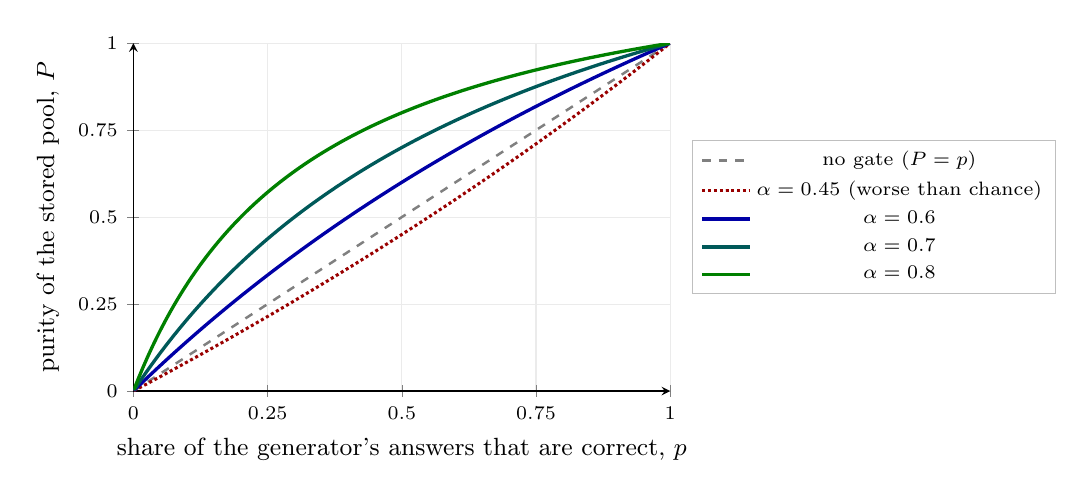
\begin{tikzpicture}
\begin{axis}[
  width=8.4cm, height=6.0cm,
  xlabel={share of the generator's answers that are correct, $p$},
  ylabel={purity of the stored pool, $P$},
  xmin=0, xmax=1, ymin=0, ymax=1,
  xtick={0,0.25,0.5,0.75,1}, ytick={0,0.25,0.5,0.75,1},
  axis lines=left, font=\small, tick label style={font=\scriptsize},
  legend style={at={(1.04,0.5)}, anchor=west, draw=black!25, font=\scriptsize, fill=white},
  grid=both, grid style={black!8}, domain=0.001:0.999, samples=120,
]
  \addplot[black!50, dashed, line width=0.9pt] {x}; \addlegendentry{no gate ($P = p$)}
  \addplot[red!60!black, line width=1.1pt, densely dotted] {0.45*x/(0.45*x + 0.55*(1-x))}; \addlegendentry{$\alpha = 0.45$ (worse than chance)}
  \addplot[blue!65!black, line width=1.2pt] {0.6*x/(0.6*x + 0.4*(1-x))}; \addlegendentry{$\alpha = 0.6$}
  \addplot[teal!70!black, line width=1.2pt] {0.7*x/(0.7*x + 0.3*(1-x))}; \addlegendentry{$\alpha = 0.7$}
  \addplot[green!50!black, line width=1.2pt] {0.8*x/(0.8*x + 0.2*(1-x))}; \addlegendentry{$\alpha = 0.8$}
\end{axis}
\end{tikzpicture}
\caption[How the purity of the stored pool depends on the gate's balanced accuracy.]{How the purity of the stored pool depends on the gate's balanced accuracy $\alpha$, from \Cref{eq:bayes-purity} with $\mathrm{TPR} = 1 - \mathrm{FPR} = \alpha$. Curves above the diagonal ($\alpha > 1/2$) make the pool purer than the generator; the dotted curve ($\alpha < 1/2$) makes it dirtier.}
\label{fig:purity-curves}
\end{figure}


Two exact consequences of \Cref{eq:bayes-purity} follow; both are about an idealised gate, not guarantees about the system.

\begin{remark}[Purity rises with the generator's accuracy]
\label{thm:monotone-purification}
For a gate with fixed $\alpha \in (0,1)$ that errs equally on both classes,
\begin{equation}
\frac{\partial P_c}{\partial p_c} \;=\; \frac{\alpha(1-\alpha)}{\big(p_c \alpha + (1-p_c)(1-\alpha)\big)^{2}} \;>\; 0,
\label{eq:monotone-purification}
\end{equation}
so a more accurate generator always yields a purer pool. (Writing $D = p_c\alpha + (1-p_c)(1-\alpha)$, the quotient rule gives $\partial P_c / \partial p_c = \alpha\,[D - p_c(2\alpha - 1)]/D^{2} = \alpha(1-\alpha)/D^{2}$.) In the run, $\alpha$ changes from cycle to cycle with the refitted composite and the range of $p_c$ is narrow, so this remark is not tested separately.
\end{remark}

\begin{remark}[Repeated filtering drives purity toward one]
\label{thm:bayes-convergence}
Suppose the stored pool were filtered again at every cycle by a gate of fixed balanced accuracy $\alpha > 1/2$ that errs equally on both classes and whose errors are independent from one pass to the next. Then the purity follows $P_{c+1} = f(P_c)$ with $f(P) = P\alpha / \big(P\alpha + (1-P)(1-\alpha)\big)$. The map $f$ is increasing, its only fixed points are $0$ and $1$, and $f(P) > P$ for every $P$ in $(0,1)$. A sequence that is increasing and bounded by one converges, and its limit must be a fixed point above $P_0$; hence $P_c \to 1$.
\end{remark}

\paragraph{How far the model is from the system:} the real loop does not re-filter the same pool with a fixed, independent gate. The composite is refitted every cycle, some verifier errors repeat at every pass, and the pool also receives new entries. The remark therefore states the direction the design aims at. Hypothesis~2, which expects purity not to fall across cycles, is tested against it in \Cref{ch:evaluation}.

\subsection{Design heuristics for the cycle-to-cycle trajectory}
\label{sec:theory-heuristics}

The five statements below describe how the pool is expected to change over cycles. Each uses at least one of three simplifications: scores that are normally distributed within the correct and incorrect classes with equal spread; a storage rate and verifier quality that stay stable across cycles; and verifier errors that are independent from one pass to the next. The real system breaks each of these (the composite is refitted every cycle, the spread of scores shrinks over cycles, and some errors are systematic), and six cycles are too few to estimate the long-run quantities involved. They are therefore heuristics, and the evaluation reads them as consistency checks.

\subsubsection{Storage-rate sensitivity}
\label{sec:theorem-monotonicity}

\begin{heuristic}[How the storage rate moves with the verifier's separation]
\label{thm:monotone}
Let $d_t$ be the Cohen's $d$ between the scores of correct and incorrect calibration-fold answers at cycle $t$, a measure of how well the verifier, seen through the cycle's refitted composite, separates them, and let $\sigma_t$ be the share of answers stored at the fixed cut-point $\tau_{\text{store}}$. Assume the scores are normal within each class with common spread $\varsigma$ and class means $\mu_{\pm} = m \pm d\,\varsigma/2$ around a fixed midpoint $m$. Let $p_{+}, p_{-}$ be the shares of correct and incorrect answers and $\phi_{\pm} = \phi\big((\mu_{\pm} - \tau_{\text{store}})/\varsigma\big)$ the class densities at the cut-point. Then $\partial \sigma / \partial d$ has the sign of $p_{+}\phi_{+} - p_{-}\phi_{-}$: when the correct class is denser at the cut-point, better separation stores more answers.
\end{heuristic}

\begin{sketch}
The storage rate is $\sigma = p_{+} \Phi\big((\mu_{+} - \tau_{\text{store}})/\varsigma\big) + p_{-} \Phi\big((\mu_{-} - \tau_{\text{store}})/\varsigma\big)$. Since $\partial \mu_{\pm}/\partial d = \pm\varsigma/2$, differentiating gives $\partial \sigma / \partial d = \tfrac12\big(p_{+}\phi_{+} - p_{-}\phi_{-}\big)$.
\end{sketch}

\paragraph{What the run shows:} the calibration fold gives four readings (cycles one, two, three and five; cycle four was rolled back). From cycle one to two, separation and storage rate moved together, as predicted; from two to three the change in $d$ was too small to read; from three to five the storage rate fell slightly while $d$ rose. Two effects outside the model explain the last case: the composite is refitted every cycle, and the spread of scores shrank rather than staying fixed. Separating them would need a cycle in which the composite is frozen and only the generator changes (\Cref{ch:conclusion}).

\subsubsection{Convergence}
\label{sec:theorem-convergence}

\begin{heuristic}[Convergence envelope]
\label{thm:convergence}
Suppose that the purity of the storage class settles to a long-run value $\pi_{\infty}$, and let $G_t = |\pi_t - \pi_{\infty}|$ be the gap at cycle $t$. Under the assumptions of \Cref{thm:purity} and \Cref{thm:monotone}, and assuming that the storage rate $\sigma$ and the separation $d$ are stable across cycles, there is a rate $r \in (0,1)$ such that, with $t$ counting only the cycles whose fine-tune was kept,
\begin{equation}
\mathbb{E}[G_{t}] \;\le\; (1-r)^{t} \, G_{0}.
\label{eq:thm-convergence}
\end{equation}
\end{heuristic}

\begin{sketch}
Each cycle adds new entries at purity $\pi_{\text{store}}$ (\Cref{thm:purity}) and re-scores the old ones. If the share of the gap closed in a cycle is roughly constant, the gap shrinks by a fixed factor $1-r$ each cycle. Under the normal model, the share closed grows with the storage rate and with the probability that the verifier ranks a correct answer above an incorrect one, $\Phi(d/\sqrt{2})$, which suggests $r$ roughly proportional to $\sigma\,\Phi(d/\sqrt{2})$. A proof would need the stochastic-approximation tools of Robbins and Monro~\cite{robbins1951stochastic}, the almost-supermartingale theorem of Robbins and Siegmund~\cite{robbins1971convergence} (used for verifier-filtered retraining by Fu et al.~\cite{fu2025collapse}) and the rate analysis of Polyak~\cite{polyak1990new}; it is left as future work.
\end{sketch}

\paragraph{What the run shows:} six cycles cannot estimate a geometric rate, so the testable reading is weaker: the calibration-fold precision stayed in a band of width $0.014$ ($0.732$ to $0.746$), comparable to the sampling noise of each reading, with no sign of drifting out of it. A direct test of the rate would need at least fifteen kept cycles under a fixed composite (\Cref{ch:conclusion}). Hypothesis~3 is tested against this heuristic in \Cref{ch:evaluation}.

\subsubsection{Asymptotic hallucination floor}
\label{sec:theorem-asymptotic}

\begin{heuristic}[Tier 1 error ceiling]
\label{cor:tier1-floor}
Let $H_{1}(t)$ be the share of wrong answers among those served by the memory-direct tier at cycle $t$. Assume that a query close enough to reach Tier 1 has the same correct answer as the stored question it matches, and that the entries Tier 1 serves are at least as often correct as the pool as a whole (plausible, because Tier 1 also requires a high stored score). Then, under \Cref{thm:purity},
\begin{equation}
\limsup_{t\to\infty}\, H_{1}(t) \;\le\; \max\!\big(1-\pi_{\text{store}},\,1-\pi_{\text{retro}}\big).
\label{eq:thm-asymptotic}
\end{equation}
\end{heuristic}

\begin{sketch}
Under the first assumption, a Tier 1 answer is wrong exactly when the stored answer is wrong; under the second, the served entries are wrong no more often than the pool, so $H_{1}(t) \le 1 - \pi_t$. By \Cref{thm:purity}, $\pi_t \ge \min(\pi_{\text{store}}, \pi_{\text{retro}})$ at every cycle, so $1 - \pi_t \le \max(1-\pi_{\text{store}}, 1-\pi_{\text{retro}})$ at every cycle, and therefore also in the limit. The first assumption is the weak point: a paraphrase that changes the answer would be served a wrong answer from a correct entry, which is why Tier 1 requires a very close match ($s \ge 0.857$).
\end{sketch}

\paragraph{What the run shows:} on the evaluation fold, whose questions never repeat stored ones, Tier 1 answered $7$ of $9{,}000$ queries, all correctly, so the ceiling cannot be observed there. The router probe of \Cref{ch:evaluation} supplies the testable case: Tier 1 answered $41$ of $42$ exact repeats and all $19$ answered paraphrases correctly. On the training panel the error rate of newly stored entries ($0.247$ to $0.276$) is close to $1 - \pi_{\text{store}}$, as assumption (ii) of \Cref{thm:purity} predicts.

\subsubsection{Equilibrium structure and self-correction}
\label{sec:theorem-corollaries}

\begin{heuristic}[Self-correction under repeated re-verification]
\label{cor:self-correction}
Consider a stored entry that is re-verified at every later cycle boundary. Assume that at each pass a correct entry survives with probability at least $\alpha$ and a wrong entry with probability at most $1-\alpha$, for a fixed $\alpha > 1/2$, and that the verdicts of different passes are independent given whether the entry is correct. Then (i) the probability that an entry is correct, given that it has survived $k$ passes, tends to one as $k$ grows; and (ii) a wrong entry is removed after at most $1/\alpha$ passes on average.
\end{heuristic}

\begin{sketch}
(i) The likelihood ratio of surviving $k$ passes for a correct versus a wrong entry is at least $\big(\alpha/(1-\alpha)\big)^{k}$, which grows without bound because $\alpha/(1-\alpha) > 1$. By Bayes' rule, $\Pr(\text{correct} \mid \text{survived } k) = \Lambda_k q / (\Lambda_k q + 1 - q)$, where $q$ is the prior probability of being correct and $\Lambda_k \ge \big(\alpha/(1-\alpha)\big)^{k}$ the likelihood ratio; this tends to one. (ii) A wrong entry is removed at each pass with probability at least $\alpha$, so the number of passes until removal is at most geometric with mean $1/\alpha$.
\end{sketch}

\paragraph{Where the assumption fails:} the independence assumption is the strong one. If the model and the verifier share a misconception, as Farquhar et al.~\cite{farquhar2024semantic} warn for systematic errors, the same wrong answer is accepted at every pass and repetition removes nothing; purity then rises only toward a ceiling set by such shared errors, which matches the finding of Fu et al.~\cite{fu2025collapse} that verifier-filtered retraining converges to the verifier's knowledge rather than to the truth. Part (ii) also shows how idealised the model is: with $\alpha > 1/2$ it predicts removal within two passes on average.

\paragraph{What the run shows:} the share of checked entries removed by the retroactive pass fell from $13$ percent at cycle one to $9$, $7$ and $4$ percent at cycles two, three and five, consistent with errors being cleared over time, though partly diluted by the growing pool of fresh entries. The entry records do not count how many passes each entry survived, so the predicted survival distribution itself could not be measured.

\begin{heuristic}[Equilibrium under retention rollback]
\label{cor:stochastic-equilibrium}
Let $X_t = 1$ if the cycle-$t$ fine-tune passes the retention guard and $X_t = 0$ if it is rolled back, and let $\pi_{\text{commit}} = \mathbb{E}[X_t]$ be the commit rate.
\begin{enumerate}[label=(\roman*)]
    \item Whenever the worst probe ratio can land on either side of the floor, $0 < \pi_{\text{commit}} < 1$.
    \item Counting all cycles, the envelope of \Cref{thm:convergence} becomes
    \begin{equation}
    \mathbb{E}[G_t] \;\le\; (1 - \pi_{\text{commit}}\, r)^{t} \, G_0,
    \label{eq:thm-stochastic-envelope}
    \end{equation}
    because a rolled-back cycle leaves the gap unchanged.
    \item The memory keeps growing through rollbacks whenever the new admissions outnumber the removals, because answering the stream chunk does not depend on $X_t$; only the adapter waits for committed cycles.
    \item When the worst probe ratio sits near the floor, commits and rollbacks alternate at a stable rate.
\end{enumerate}
\end{heuristic}

\begin{sketch}
A committed cycle shrinks the expected gap by the factor $1-r$ and a rolled-back cycle leaves it unchanged, so $\mathbb{E}[G_{t+1} \mid G_t] = (1 - \pi_{\text{commit}}\, r)\, G_t$; iterating gives \Cref{eq:thm-stochastic-envelope}. Part (iii) follows from the fact that the stream chunk is answered, and new entries stored, whether or not the cycle's fine-tune is kept. Part (iv) is an informal claim about a stationary state and is not proven.
\end{sketch}

\paragraph{What the run shows:} parts (i) and (iii) can be checked directly. The commit sequence over cycles one to five was $1, 1, 1, 0, 1$, with worst probe ratios $1.006$, $0.949$, $0.976$, $0.886$ and $0.958$, so the observed commit rate is $4/5$. The memory grew at every cycle, including across the cycle-four rollback (\Cref{tab:app-per-cycle-memory}). Part (ii) inherits the limits of \Cref{thm:convergence}, and part (iv) would need at least fifteen kept cycles to test (\Cref{ch:conclusion}); the ratios at cycles two to five lie within $0.07$ of the floor, which is consistent with it but not evidence for it.

\subsection{Remarks on the overall hallucination rate}
\label{sec:theorem-scaffolding}

Two further remarks place the memory's contribution within the error rate of the whole system. Neither is measured in this thesis.

\begin{remark}[Decomposition of the overall error rate]
\label{thm:asymptotic-elim}
Let $\tau_{1}(t)$ be the share of queries answered by Tier 1 at cycle $t$, $H_{\text{mem}}(t)$ the error rate of those answers (at most $1 - \pi_t$ under the assumptions of \Cref{cor:tier1-floor}), and $H_{\text{gen}}(t)$ the error rate of answers generated by Tiers 2 and 3. By the law of total probability, the overall error rate is
\begin{equation}
H_t \;=\; \big(1 - \tau_{1}(t)\big) \, H_{\text{gen}}(t) \;+\; \tau_{1}(t) \, H_{\text{mem}}(t).
\label{eq:asymptotic-elim}
\end{equation}
The memory can lower the overall rate only through the second term, so its effect grows with the share of queries it answers. As $\pi_t$ rises, the bound on $H_{\text{mem}}$ falls, and the remaining error is set by the generator and its retrieval corpus on the questions the memory cannot answer.
\end{remark}

\paragraph{Reading the remark:} on the evaluation fold $\tau_{1}(t)$ was at most $0.1$ percent, so the overall rate there is essentially the generator's. The remark becomes testable only in deployment, where real users repeat questions; Hypothesis~4 is read against it in \Cref{ch:evaluation}.

\begin{remark}[Ceiling set by the retrieval corpus]
\label{cor:corpus-floor}
Let $K(C)$ be the set of questions whose answer can be supported by the corpus $C$. A system that answers every question and asserts only what $C$ supports can be right on at most the questions in $K(C)$; on the rest any answer it gives is wrong, so it must abstain or err. The error left after the memory and the generator have done their best is therefore bounded below by the share of questions outside $K(C)$ that the system chooses to answer, a limit set by the corpus rather than by the architecture. Estimating it would require checking, for every evaluation question, whether any retrieved passage contains the gold answer, which was not done (\Cref{ch:conclusion}).
\end{remark}

\section{Chapter signpost}
\label{sec:ch4-signpost}

This chapter fixed every component, threshold and fitting procedure before the results were read. \Cref{ch:evaluation} measures them on the six-cycle run, the eight external baselines and the retrieval-utility-classifier comparison; it reports each pre-specified hypothesis as supported, partly supported or unsupported, checks the two proven results against their measurements, and reads the heuristics as consistency checks.
